% Options for packages loaded elsewhere
\PassOptionsToPackage{unicode}{hyperref}
\PassOptionsToPackage{hyphens}{url}
%
\documentclass[
]{article}
\usepackage{amsmath,amssymb}
\usepackage{lmodern}
\usepackage{iftex}
\ifPDFTeX
  \usepackage[T1]{fontenc}
  \usepackage[utf8]{inputenc}
  \usepackage{textcomp} % provide euro and other symbols
\else % if luatex or xetex
  \usepackage{unicode-math}
  \defaultfontfeatures{Scale=MatchLowercase}
  \defaultfontfeatures[\rmfamily]{Ligatures=TeX,Scale=1}
\fi
% Use upquote if available, for straight quotes in verbatim environments
\IfFileExists{upquote.sty}{\usepackage{upquote}}{}
\IfFileExists{microtype.sty}{% use microtype if available
  \usepackage[]{microtype}
  \UseMicrotypeSet[protrusion]{basicmath} % disable protrusion for tt fonts
}{}
\makeatletter
\@ifundefined{KOMAClassName}{% if non-KOMA class
  \IfFileExists{parskip.sty}{%
    \usepackage{parskip}
  }{% else
    \setlength{\parindent}{0pt}
    \setlength{\parskip}{6pt plus 2pt minus 1pt}}
}{% if KOMA class
  \KOMAoptions{parskip=half}}
\makeatother
\usepackage{xcolor}
\usepackage[margin=1in]{geometry}
\usepackage{color}
\usepackage{fancyvrb}
\newcommand{\VerbBar}{|}
\newcommand{\VERB}{\Verb[commandchars=\\\{\}]}
\DefineVerbatimEnvironment{Highlighting}{Verbatim}{commandchars=\\\{\}}
% Add ',fontsize=\small' for more characters per line
\usepackage{framed}
\definecolor{shadecolor}{RGB}{248,248,248}
\newenvironment{Shaded}{\begin{snugshade}}{\end{snugshade}}
\newcommand{\AlertTok}[1]{\textcolor[rgb]{0.94,0.16,0.16}{#1}}
\newcommand{\AnnotationTok}[1]{\textcolor[rgb]{0.56,0.35,0.01}{\textbf{\textit{#1}}}}
\newcommand{\AttributeTok}[1]{\textcolor[rgb]{0.77,0.63,0.00}{#1}}
\newcommand{\BaseNTok}[1]{\textcolor[rgb]{0.00,0.00,0.81}{#1}}
\newcommand{\BuiltInTok}[1]{#1}
\newcommand{\CharTok}[1]{\textcolor[rgb]{0.31,0.60,0.02}{#1}}
\newcommand{\CommentTok}[1]{\textcolor[rgb]{0.56,0.35,0.01}{\textit{#1}}}
\newcommand{\CommentVarTok}[1]{\textcolor[rgb]{0.56,0.35,0.01}{\textbf{\textit{#1}}}}
\newcommand{\ConstantTok}[1]{\textcolor[rgb]{0.00,0.00,0.00}{#1}}
\newcommand{\ControlFlowTok}[1]{\textcolor[rgb]{0.13,0.29,0.53}{\textbf{#1}}}
\newcommand{\DataTypeTok}[1]{\textcolor[rgb]{0.13,0.29,0.53}{#1}}
\newcommand{\DecValTok}[1]{\textcolor[rgb]{0.00,0.00,0.81}{#1}}
\newcommand{\DocumentationTok}[1]{\textcolor[rgb]{0.56,0.35,0.01}{\textbf{\textit{#1}}}}
\newcommand{\ErrorTok}[1]{\textcolor[rgb]{0.64,0.00,0.00}{\textbf{#1}}}
\newcommand{\ExtensionTok}[1]{#1}
\newcommand{\FloatTok}[1]{\textcolor[rgb]{0.00,0.00,0.81}{#1}}
\newcommand{\FunctionTok}[1]{\textcolor[rgb]{0.00,0.00,0.00}{#1}}
\newcommand{\ImportTok}[1]{#1}
\newcommand{\InformationTok}[1]{\textcolor[rgb]{0.56,0.35,0.01}{\textbf{\textit{#1}}}}
\newcommand{\KeywordTok}[1]{\textcolor[rgb]{0.13,0.29,0.53}{\textbf{#1}}}
\newcommand{\NormalTok}[1]{#1}
\newcommand{\OperatorTok}[1]{\textcolor[rgb]{0.81,0.36,0.00}{\textbf{#1}}}
\newcommand{\OtherTok}[1]{\textcolor[rgb]{0.56,0.35,0.01}{#1}}
\newcommand{\PreprocessorTok}[1]{\textcolor[rgb]{0.56,0.35,0.01}{\textit{#1}}}
\newcommand{\RegionMarkerTok}[1]{#1}
\newcommand{\SpecialCharTok}[1]{\textcolor[rgb]{0.00,0.00,0.00}{#1}}
\newcommand{\SpecialStringTok}[1]{\textcolor[rgb]{0.31,0.60,0.02}{#1}}
\newcommand{\StringTok}[1]{\textcolor[rgb]{0.31,0.60,0.02}{#1}}
\newcommand{\VariableTok}[1]{\textcolor[rgb]{0.00,0.00,0.00}{#1}}
\newcommand{\VerbatimStringTok}[1]{\textcolor[rgb]{0.31,0.60,0.02}{#1}}
\newcommand{\WarningTok}[1]{\textcolor[rgb]{0.56,0.35,0.01}{\textbf{\textit{#1}}}}
\usepackage{graphicx}
\makeatletter
\def\maxwidth{\ifdim\Gin@nat@width>\linewidth\linewidth\else\Gin@nat@width\fi}
\def\maxheight{\ifdim\Gin@nat@height>\textheight\textheight\else\Gin@nat@height\fi}
\makeatother
% Scale images if necessary, so that they will not overflow the page
% margins by default, and it is still possible to overwrite the defaults
% using explicit options in \includegraphics[width, height, ...]{}
\setkeys{Gin}{width=\maxwidth,height=\maxheight,keepaspectratio}
% Set default figure placement to htbp
\makeatletter
\def\fps@figure{htbp}
\makeatother
\setlength{\emergencystretch}{3em} % prevent overfull lines
\providecommand{\tightlist}{%
  \setlength{\itemsep}{0pt}\setlength{\parskip}{0pt}}
\setcounter{secnumdepth}{-\maxdimen} % remove section numbering
\ifLuaTeX
  \usepackage{selnolig}  % disable illegal ligatures
\fi
\IfFileExists{bookmark.sty}{\usepackage{bookmark}}{\usepackage{hyperref}}
\IfFileExists{xurl.sty}{\usepackage{xurl}}{} % add URL line breaks if available
\urlstyle{same} % disable monospaced font for URLs
\hypersetup{
  pdftitle={IODS},
  pdfauthor={Rong Guang},
  hidelinks,
  pdfcreator={LaTeX via pandoc}}

\title{IODS}
\usepackage{etoolbox}
\makeatletter
\providecommand{\subtitle}[1]{% add subtitle to \maketitle
  \apptocmd{\@title}{\par {\large #1 \par}}{}{}
}
\makeatother
\subtitle{Chapter 4}
\author{Rong Guang}
\date{22/11/2022}

\begin{document}
\maketitle

{
\setcounter{tocdepth}{3}
\tableofcontents
}
\hypertarget{chapter-4-clustering}{%
\section{\texorpdfstring{\textbf{Chapter 4:
Clustering}}{Chapter 4: Clustering}}\label{chapter-4-clustering}}

\hypertarget{create-a-new-r-markdown-file-and-save-it-as-an-empty-file-named-chapter4.rmd.-then-include-the-file-as-a-child-file-in-your-index.rmd-file.}{%
\subsection{1 Create a new R Markdown file and save it as an empty file
named `chapter4.Rmd'. Then include the file as a child file in your
`index.Rmd'
file.}\label{create-a-new-r-markdown-file-and-save-it-as-an-empty-file-named-chapter4.rmd.-then-include-the-file-as-a-child-file-in-your-index.rmd-file.}}

\hypertarget{create-a-new-r-markdown-file-and-save-it-as-an-empty-file-named-chapter4.rmd}{%
\subsubsection{1.1 Create a new R Markdown file and save it as an empty
file named
`chapter4.Rmd'}\label{create-a-new-r-markdown-file-and-save-it-as-an-empty-file-named-chapter4.rmd}}

Done!

\hypertarget{include-the-file-as-a-child-file-in-your-index.rmd-file.}{%
\subsubsection{1.2 include the file as a child file in your `index.Rmd'
file.}\label{include-the-file-as-a-child-file-in-your-index.rmd-file.}}

Done!

\hypertarget{load-the-boston-data-from-the-mass-package.-explore-the-structure-and-the-dimensions-of-the-data-and-describe-the-dataset-briefly-assuming-the-reader-has-no-previous-knowledge-of-it.-0-1-points}{%
\subsection{2 Load the Boston data from the MASS package. Explore the
structure and the dimensions of the data and describe the dataset
briefly, assuming the reader has no previous knowledge of it. (0-1
points)}\label{load-the-boston-data-from-the-mass-package.-explore-the-structure-and-the-dimensions-of-the-data-and-describe-the-dataset-briefly-assuming-the-reader-has-no-previous-knowledge-of-it.-0-1-points}}

\hypertarget{load-the-boston-data-from-the-mass-package.}{%
\subsubsection{2.1 Load the Boston data from the MASS
package.}\label{load-the-boston-data-from-the-mass-package.}}

\begin{Shaded}
\begin{Highlighting}[]
\CommentTok{\# access the MASS package}
\FunctionTok{library}\NormalTok{(MASS)}

\CommentTok{\# load the data}
\FunctionTok{data}\NormalTok{(}\StringTok{"Boston"}\NormalTok{)}

\CommentTok{\# pass Boston to another object for easy typing}
\NormalTok{bos }\OtherTok{\textless{}{-}}\NormalTok{ Boston}
\end{Highlighting}
\end{Shaded}

\hypertarget{explore-the-structure-and-the-dimensions-of-the-data}{%
\subsubsection{2.2 Explore the structure and the dimensions of the
data}\label{explore-the-structure-and-the-dimensions-of-the-data}}

\begin{Shaded}
\begin{Highlighting}[]
\FunctionTok{library}\NormalTok{(tidyverse)}
\end{Highlighting}
\end{Shaded}

\begin{verbatim}
## -- Attaching packages --------------------------------------- tidyverse 1.3.2 --
## v ggplot2 3.3.6     v purrr   0.3.4
## v tibble  3.1.6     v dplyr   1.0.8
## v tidyr   1.2.0     v stringr 1.4.0
## v readr   2.1.2     v forcats 0.5.1
## -- Conflicts ------------------------------------------ tidyverse_conflicts() --
## x dplyr::filter() masks stats::filter()
## x dplyr::lag()    masks stats::lag()
## x dplyr::select() masks MASS::select()
\end{verbatim}

\begin{Shaded}
\begin{Highlighting}[]
\CommentTok{\#explore structure}
\FunctionTok{str}\NormalTok{(bos)}
\end{Highlighting}
\end{Shaded}

\begin{verbatim}
## 'data.frame':    506 obs. of  14 variables:
##  $ crim   : num  0.00632 0.02731 0.02729 0.03237 0.06905 ...
##  $ zn     : num  18 0 0 0 0 0 12.5 12.5 12.5 12.5 ...
##  $ indus  : num  2.31 7.07 7.07 2.18 2.18 2.18 7.87 7.87 7.87 7.87 ...
##  $ chas   : int  0 0 0 0 0 0 0 0 0 0 ...
##  $ nox    : num  0.538 0.469 0.469 0.458 0.458 0.458 0.524 0.524 0.524 0.524 ...
##  $ rm     : num  6.58 6.42 7.18 7 7.15 ...
##  $ age    : num  65.2 78.9 61.1 45.8 54.2 58.7 66.6 96.1 100 85.9 ...
##  $ dis    : num  4.09 4.97 4.97 6.06 6.06 ...
##  $ rad    : int  1 2 2 3 3 3 5 5 5 5 ...
##  $ tax    : num  296 242 242 222 222 222 311 311 311 311 ...
##  $ ptratio: num  15.3 17.8 17.8 18.7 18.7 18.7 15.2 15.2 15.2 15.2 ...
##  $ black  : num  397 397 393 395 397 ...
##  $ lstat  : num  4.98 9.14 4.03 2.94 5.33 ...
##  $ medv   : num  24 21.6 34.7 33.4 36.2 28.7 22.9 27.1 16.5 18.9 ...
\end{verbatim}

\begin{Shaded}
\begin{Highlighting}[]
\CommentTok{\#explore dimensions}
\FunctionTok{dim}\NormalTok{(bos)}
\end{Highlighting}
\end{Shaded}

\begin{verbatim}
## [1] 506  14
\end{verbatim}

\begin{Shaded}
\begin{Highlighting}[]
\CommentTok{\#generate a codebook}
\CommentTok{\# string is copy from dataset introduction}
\NormalTok{codebook }\OtherTok{\textless{}{-}} \FunctionTok{data.frame}\NormalTok{(}\AttributeTok{variable =} \StringTok{"CRIM {-} per capita crime rate by town/ZN {-} proportion of residential land zoned for lots over 25,000 sq.ft./INDUS {-} proportion of non{-}retail business acres per town./CHAS {-} Charles River dummy variable (1 if tract bounds river; 0 otherwise)/NOX {-} nitric oxides concentration (parts per 10 million)/RM {-} average number of rooms per dwelling/AGE {-} proportion of owner{-}occupied units built prior to 1940/DIS {-} weighted distances to five Boston employment centres/RAD {-} index of accessibility to radial highways/TAX {-} full{-}value property{-}tax rate per $10,000/PTRATIO {-} pupil{-}teacher ratio by town/B {-} 1000(Bk{-}0.63)\^{}2 where Bk is the proportion of blacks by town/LSTAT {-} \% lower status of the population/MEDV {-} Median value of owner{-}occupied homes in $1000\textquotesingle{}s"}\NormalTok{) }

\NormalTok{codebook }\OtherTok{\textless{}{-}}\NormalTok{ codebook }\SpecialCharTok{\%\textgreater{}\%} 
  \FunctionTok{separate\_rows}\NormalTok{(variable, }\AttributeTok{sep =} \StringTok{"/"}\NormalTok{) }\SpecialCharTok{\%\textgreater{}\%}  \CommentTok{\# "/" is the delimiter for rows}
  \FunctionTok{separate}\NormalTok{(variable, }\AttributeTok{sep =} \StringTok{" {-} "}\NormalTok{,      }\CommentTok{\#" {-} " is the delimiter for variables}
           \AttributeTok{into =} \FunctionTok{c}\NormalTok{(}\StringTok{"name"}\NormalTok{, }\StringTok{"description"}\NormalTok{),  }\CommentTok{\# names of sparated variables}
           \AttributeTok{remove =}\NormalTok{ T)  }\CommentTok{\#remove old column}
\CommentTok{\#check codebook}
\FunctionTok{library}\NormalTok{(DT)}
\NormalTok{codebook }\SpecialCharTok{\%\textgreater{}\%}\NormalTok{ datatable }
\end{Highlighting}
\end{Shaded}

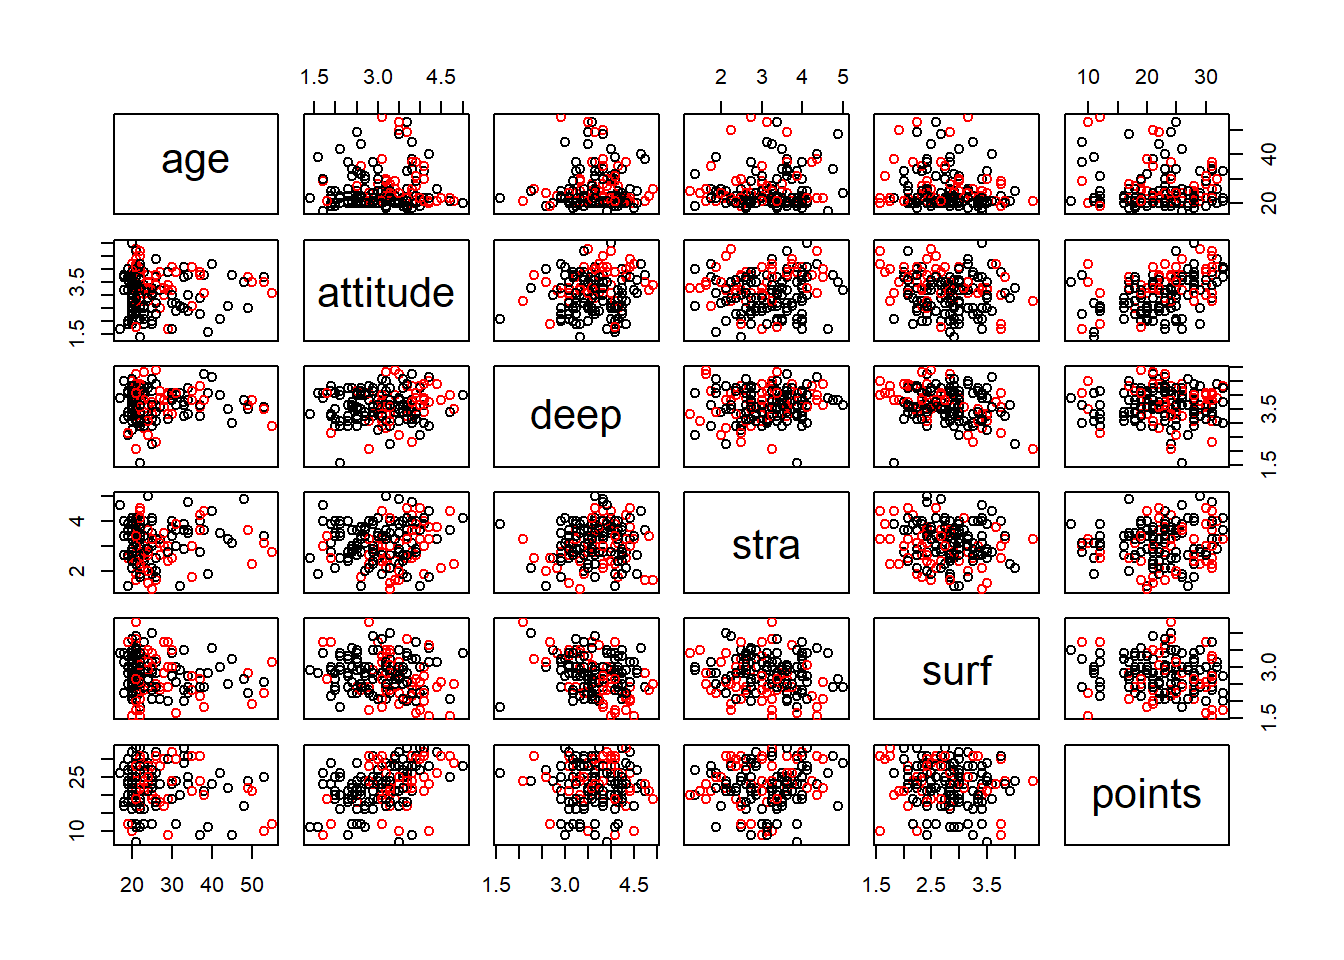
\includegraphics{chapter4_files/figure-latex/unnamed-chunk-2-1.pdf}

The data set has 506 observations of 14 variables. Variable CHAS is a
dummy variable where 1 means the the place having tract that bounds
river, and 0 means otherwise. It needs to be converted to a factor.

\begin{Shaded}
\begin{Highlighting}[]
\NormalTok{bos }\OtherTok{\textless{}{-}}\NormalTok{ bos }\SpecialCharTok{\%\textgreater{}\%} 
  \FunctionTok{mutate}\NormalTok{(}\AttributeTok{chas =}\NormalTok{ chas }\SpecialCharTok{\%\textgreater{}\%}
           \FunctionTok{factor}\NormalTok{() }\SpecialCharTok{\%\textgreater{}\%} 
           \FunctionTok{fct\_recode}\NormalTok{(}
             \StringTok{"With tracts that bonds river"} \OtherTok{=} \StringTok{"1"}\NormalTok{, }\CommentTok{\#old value 1 to new label}
             \StringTok{"Otherwise"} \OtherTok{=} \StringTok{"0"}\NormalTok{) }\CommentTok{\# old value 0 to new label}
\NormalTok{)}
\end{Highlighting}
\end{Shaded}

\hypertarget{describe-the-dataset}{%
\subsubsection{2.3 describe the dataset}\label{describe-the-dataset}}

Each of the 506 rows in the dataset describes a Boston suburb or town,
and it has 14 columns with information such as average number of rooms
per dwelling, pupil-teacher ratio, and per capita crime rate. The last
row describes the median price of owner-occupied homes.

\hypertarget{show-a-graphical-overview-of-the-data-and-show-summaries-of-the-variables-in-the-data.-describe-and-interpret-the-outputs-commenting-on-the-distributions-of-the-variables-and-the-relationships-between-them.-0-2-points}{%
\subsection{3 Show a graphical overview of the data and show summaries
of the variables in the data. Describe and interpret the outputs,
commenting on the distributions of the variables and the relationships
between them. (0-2
points)}\label{show-a-graphical-overview-of-the-data-and-show-summaries-of-the-variables-in-the-data.-describe-and-interpret-the-outputs-commenting-on-the-distributions-of-the-variables-and-the-relationships-between-them.-0-2-points}}

\hypertarget{show-a-graphical-overview-of-the-data}{%
\subsubsection{3.1 Show a graphical overview of the
data}\label{show-a-graphical-overview-of-the-data}}

\begin{Shaded}
\begin{Highlighting}[]
\FunctionTok{library}\NormalTok{(GGally)}
\end{Highlighting}
\end{Shaded}

\begin{verbatim}
## Registered S3 method overwritten by 'GGally':
##   method from   
##   +.gg   ggplot2
\end{verbatim}

\begin{Shaded}
\begin{Highlighting}[]
\FunctionTok{library}\NormalTok{(ggplot2)}

\CommentTok{\#define a function that allows me to fine{-}tune the matrix}
\NormalTok{my.fun }\OtherTok{\textless{}{-}} \ControlFlowTok{function}\NormalTok{(data, mapping, }\AttributeTok{method =} \StringTok{"lm"}\NormalTok{,...)\{ }\CommentTok{\#define arguments}
\NormalTok{  p }\OtherTok{\textless{}{-}} \FunctionTok{ggplot}\NormalTok{(}\AttributeTok{data =}\NormalTok{ data, }\AttributeTok{mapping =}\NormalTok{ mapping) }\SpecialCharTok{+} \CommentTok{\#pass arguments}
    \FunctionTok{geom\_point}\NormalTok{(}\AttributeTok{size =} \FloatTok{0.3}\NormalTok{, }
               \AttributeTok{color =} \StringTok{"blue"}\NormalTok{,...) }\SpecialCharTok{+} \CommentTok{\#define points size and color}
    \FunctionTok{geom\_smooth}\NormalTok{(}\AttributeTok{size =} \FloatTok{0.5}\NormalTok{, }
                \AttributeTok{color =} \StringTok{"red"}\NormalTok{, }
                \AttributeTok{method =}\NormalTok{ method) }\CommentTok{\#define line size and color; define lm regression}
\NormalTok{  p }\CommentTok{\#print the results}
\NormalTok{\}}

\CommentTok{\#the abbreviated variable names are not self{-}explanatory, set column and row}
\CommentTok{\#names to be the variable labels for better reading}
\CommentTok{\#this new object will be used in ggpairs function}
\NormalTok{names1 }\OtherTok{\textless{}{-}} \FunctionTok{pull}\NormalTok{(codebook[}\DecValTok{1}\SpecialCharTok{:}\DecValTok{7}\NormalTok{,], description)  }\CommentTok{\# extract row 1:7 of var description}
\NormalTok{names1 }\OtherTok{\textless{}{-}} \FunctionTok{sapply}\NormalTok{(names1,    }\CommentTok{\#collapse the description into multiple lines}
                 \ControlFlowTok{function}\NormalTok{(x) }\FunctionTok{paste}\NormalTok{(}\FunctionTok{strwrap}\NormalTok{(x, }\DecValTok{35}\NormalTok{),  }\CommentTok{\# for better reading}
                                   \AttributeTok{collapse =} \StringTok{"}\SpecialCharTok{\textbackslash{}n}\StringTok{"}\NormalTok{)) }\CommentTok{\# "\textbackslash{}n" calls for a new line}

\FunctionTok{ggpairs}\NormalTok{(bos, }
        \AttributeTok{lower =} \FunctionTok{list}\NormalTok{(}
          \AttributeTok{continuous =}\NormalTok{ my.fun,}
          \AttributeTok{combo =} \FunctionTok{wrap}\NormalTok{(}\StringTok{"facethist"}\NormalTok{, }\AttributeTok{bins =} \DecValTok{20}\NormalTok{)),}
        \AttributeTok{col =} \DecValTok{1}\SpecialCharTok{:}\DecValTok{7}\NormalTok{,}
        \AttributeTok{columnLabels =}\NormalTok{ names1) }\CommentTok{\#define column labels as the names I just set}
\end{Highlighting}
\end{Shaded}

\begin{verbatim}
## `geom_smooth()` using formula 'y ~ x'
\end{verbatim}

\begin{verbatim}
## `geom_smooth()` using formula 'y ~ x'
## `geom_smooth()` using formula 'y ~ x'
## `geom_smooth()` using formula 'y ~ x'
## `geom_smooth()` using formula 'y ~ x'
## `geom_smooth()` using formula 'y ~ x'
## `geom_smooth()` using formula 'y ~ x'
## `geom_smooth()` using formula 'y ~ x'
## `geom_smooth()` using formula 'y ~ x'
## `geom_smooth()` using formula 'y ~ x'
## `geom_smooth()` using formula 'y ~ x'
## `geom_smooth()` using formula 'y ~ x'
## `geom_smooth()` using formula 'y ~ x'
## `geom_smooth()` using formula 'y ~ x'
## `geom_smooth()` using formula 'y ~ x'
\end{verbatim}

\begin{figure}
\centering
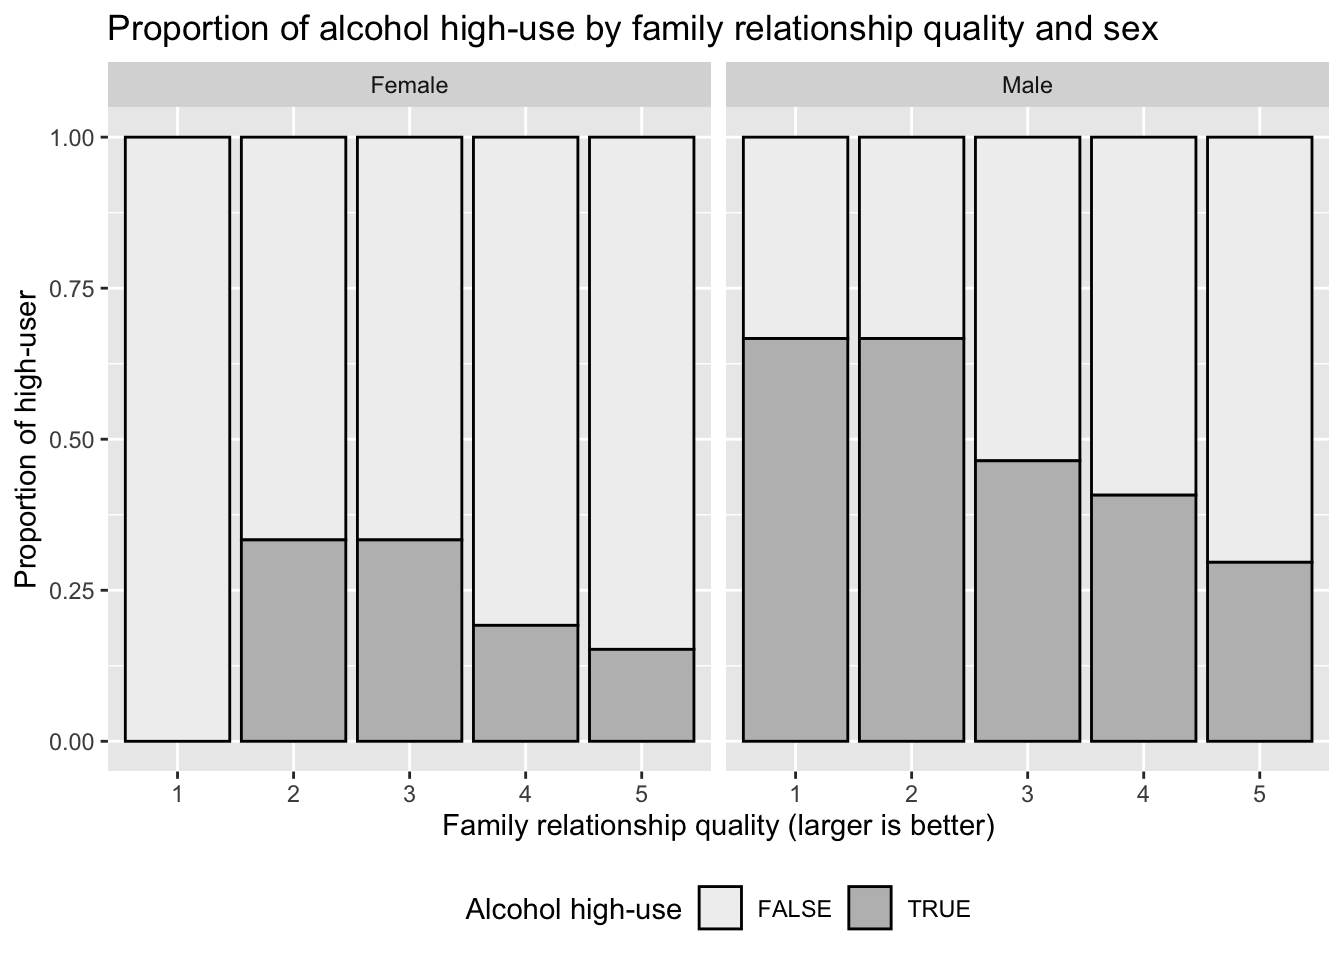
\includegraphics{chapter4_files/figure-latex/unnamed-chunk-4-1.pdf}
\caption{Visualized relations of Boston dataset, variable
\#1\textasciitilde\#7}
\end{figure}

Note that variable about crime rate is plagued with outliers.

\begin{Shaded}
\begin{Highlighting}[]
\CommentTok{\#repeat what is done in the last chunk for variable 8\textasciitilde{}14}
\NormalTok{names2 }\OtherTok{\textless{}{-}} \FunctionTok{pull}\NormalTok{(codebook[}\DecValTok{8}\SpecialCharTok{:}\DecValTok{14}\NormalTok{,], description)}
\NormalTok{names2 }\OtherTok{\textless{}{-}} \FunctionTok{sapply}\NormalTok{(names1, }\ControlFlowTok{function}\NormalTok{(x) }\FunctionTok{paste}\NormalTok{(}\FunctionTok{strwrap}\NormalTok{(x, }\DecValTok{35}\NormalTok{), }\AttributeTok{collapse =} \StringTok{"}\SpecialCharTok{\textbackslash{}n}\StringTok{"}\NormalTok{))}

\FunctionTok{ggpairs}\NormalTok{(bos, }
        \AttributeTok{lower =} \FunctionTok{list}\NormalTok{(}
          \AttributeTok{continuous =}\NormalTok{ my.fun),}
        \AttributeTok{col =} \DecValTok{8}\SpecialCharTok{:}\DecValTok{14}\NormalTok{,}
        \AttributeTok{columnLabels =}\NormalTok{ names2,}
\NormalTok{        )}
\end{Highlighting}
\end{Shaded}

\begin{verbatim}
## `geom_smooth()` using formula 'y ~ x'
## `geom_smooth()` using formula 'y ~ x'
## `geom_smooth()` using formula 'y ~ x'
## `geom_smooth()` using formula 'y ~ x'
## `geom_smooth()` using formula 'y ~ x'
## `geom_smooth()` using formula 'y ~ x'
## `geom_smooth()` using formula 'y ~ x'
## `geom_smooth()` using formula 'y ~ x'
## `geom_smooth()` using formula 'y ~ x'
## `geom_smooth()` using formula 'y ~ x'
## `geom_smooth()` using formula 'y ~ x'
## `geom_smooth()` using formula 'y ~ x'
## `geom_smooth()` using formula 'y ~ x'
## `geom_smooth()` using formula 'y ~ x'
## `geom_smooth()` using formula 'y ~ x'
## `geom_smooth()` using formula 'y ~ x'
## `geom_smooth()` using formula 'y ~ x'
## `geom_smooth()` using formula 'y ~ x'
## `geom_smooth()` using formula 'y ~ x'
## `geom_smooth()` using formula 'y ~ x'
## `geom_smooth()` using formula 'y ~ x'
\end{verbatim}

\begin{figure}
\centering
\includegraphics{chapter4_files/figure-latex/unnamed-chunk-5-1.pdf}
\caption{Visualized relations of Boston dataset, variable
\#8\textasciitilde\#14}
\end{figure}

\hypertarget{show-summaries-of-the-variables-in-the-data.}{%
\subsubsection{3.2 Show summaries of the variables in the
data.}\label{show-summaries-of-the-variables-in-the-data.}}

\begin{Shaded}
\begin{Highlighting}[]
\FunctionTok{library}\NormalTok{(finalfit)}
\CommentTok{\#summarize the continuous data}
\FunctionTok{ff\_glimpse}\NormalTok{(bos)}\SpecialCharTok{$}\NormalTok{Continuous }\SpecialCharTok{\%\textgreater{}\%}\NormalTok{ datatable}
\end{Highlighting}
\end{Shaded}

\includegraphics{chapter4_files/figure-latex/unnamed-chunk-6-1.pdf}

\begin{Shaded}
\begin{Highlighting}[]
\CommentTok{\# summarize the categorical data}
\FunctionTok{ff\_glimpse}\NormalTok{(bos)}\SpecialCharTok{$}\NormalTok{Categorical }\SpecialCharTok{\%\textgreater{}\%}\NormalTok{ datatable}
\end{Highlighting}
\end{Shaded}

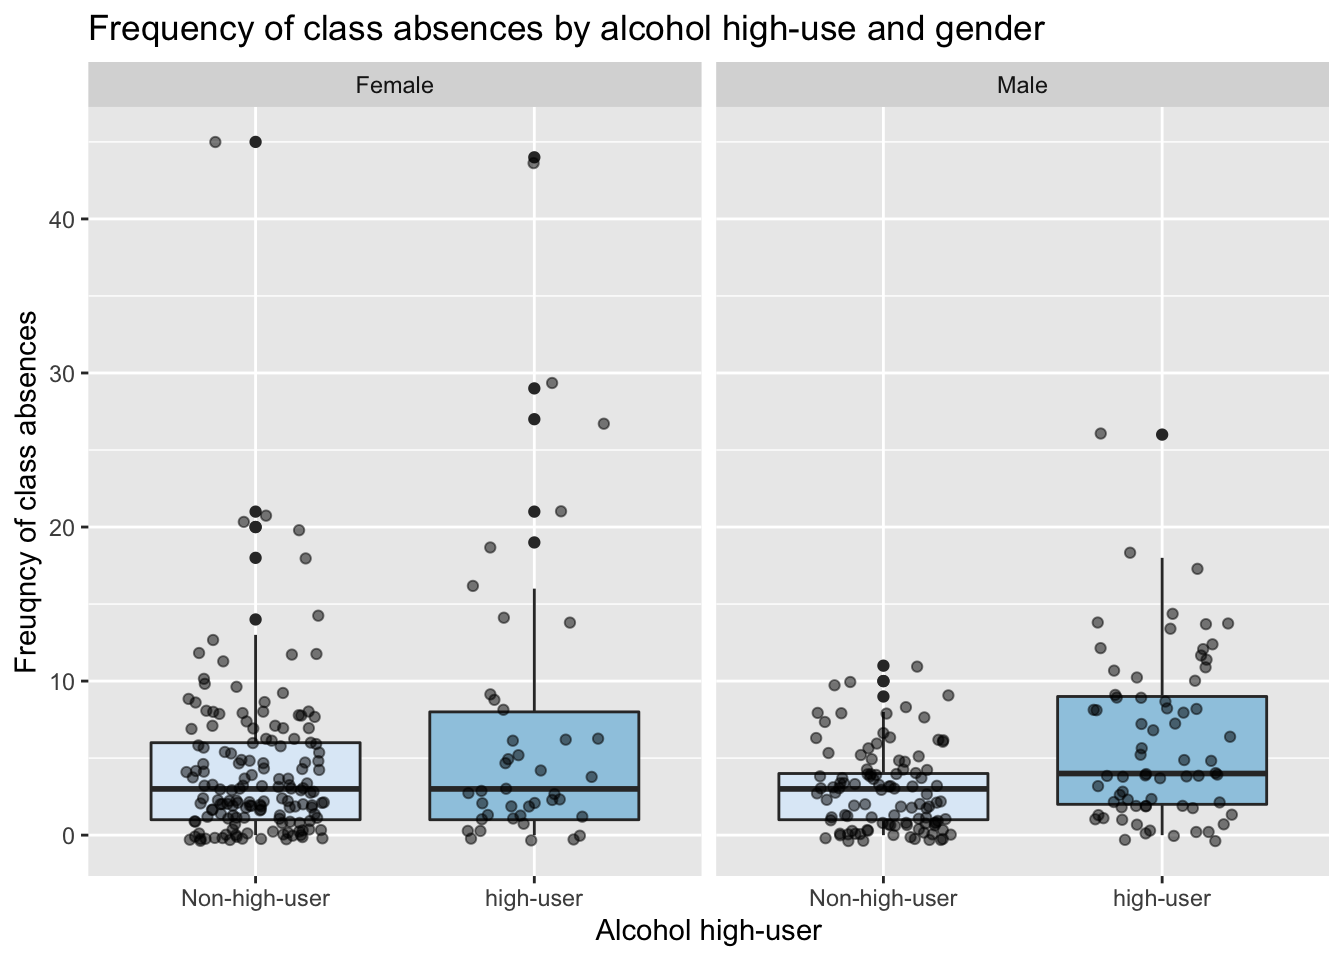
\includegraphics{chapter4_files/figure-latex/unnamed-chunk-7-1.pdf}

\hypertarget{describe-and-interpret-the-outputs-commenting-on-the-distributions-of-the-variables-and-the-relationships-between-them.}{%
\subsubsection{3.3 Describe and interpret the outputs, commenting on the
distributions of the variables and the relationships between
them.}\label{describe-and-interpret-the-outputs-commenting-on-the-distributions-of-the-variables-and-the-relationships-between-them.}}

\hypertarget{interpreting-continuous-variables}{%
\paragraph{3.3.1 interpreting continuous
variables}\label{interpreting-continuous-variables}}

There are 13 continuous variables in the dataset. The crime rate of the
town was 0.3(0.1\textasciitilde3.7)\%; the proportion of a town's
residential land zoned for lots over 25,000 sq.ft. was 0
(0\textasciitilde12.5)\%; the proportion of non-retail business acres
per town was 9.7(5.2\textasciitilde18.1)\%; the nitric oxides
concentration was 0.5(0.4\textasciitilde0.6) parts per 10 million; the
average number of rooms per dwelling was 6.3±0.7 rooms; the proportion
of owner-occupied units built prior to 1940 was
77.5(45.0\textasciitilde94.1)\%; the weighted distances to five Boston
employment centres was 3.2 (2.1\textasciitilde5.2) kilometers; the index
of accessibility to radial highways was 5(4\textasciitilde24) units of
accessibility; the full-value property-tax rate was
\$330(279\textasciitilde666) per \$10,000; the pupil-teacher ratio by
town was 19.1(17.4\textasciitilde20.2); the Black proportion of
population after taking the formula of 1000(Bk-0.63)\^{}2 was
391.4(375.4\textasciitilde396.2); the proportion of population that is
lower status was 11.4(6.9\textasciitilde17.0)\%; the median value of
owner-occupied homes was \$21.2(17\textasciitilde25)*1000. \#\#\#\#
3.3.2 interpreting categorical variable

35(6.9\%) towns have tracts that bonds Charles River.

\hypertarget{commenting-on-the-relationships-between-variables}{%
\paragraph{3.3.3 commenting on the relationships between
variables}\label{commenting-on-the-relationships-between-variables}}

Except for the one binary variable about tract that bonds river, each
variable in our data set shows a \textgreater0.3 and/or \textless-0.3
correlation with at least one of the other variables. Some of them have
correlation as high as 0.9. All of the correlation coefficients are
significant (\emph{p}\textless0.001).

\hypertarget{standardize-the-dataset-and-print-out-summaries-of-the-scaled-data.-how-did-the-variables-change-create-a-categorical-variable-of-the-crime-rate-in-the-boston-dataset-from-the-scaled-crime-rate.-use-the-quantiles-as-the-break-points-in-the-categorical-variable.-drop-the-old-crime-rate-variable-from-the-dataset.-divide-the-dataset-to-train-and-test-sets-so-that-80-of-the-data-belongs-to-the-train-set.-0-2-points}{%
\subsection{4 Standardize the dataset and print out summaries of the
scaled data. How did the variables change? Create a categorical variable
of the crime rate in the Boston dataset (from the scaled crime rate).
Use the quantiles as the break points in the categorical variable. Drop
the old crime rate variable from the dataset. Divide the dataset to
train and test sets, so that 80\% of the data belongs to the train set.
(0-2
points)}\label{standardize-the-dataset-and-print-out-summaries-of-the-scaled-data.-how-did-the-variables-change-create-a-categorical-variable-of-the-crime-rate-in-the-boston-dataset-from-the-scaled-crime-rate.-use-the-quantiles-as-the-break-points-in-the-categorical-variable.-drop-the-old-crime-rate-variable-from-the-dataset.-divide-the-dataset-to-train-and-test-sets-so-that-80-of-the-data-belongs-to-the-train-set.-0-2-points}}

\hypertarget{standardize-the-dataset-and-print-out-summaries-of-the-scaled-data}{%
\subsubsection{4.1 Standardize the dataset and print out summaries of
the scaled
data}\label{standardize-the-dataset-and-print-out-summaries-of-the-scaled-data}}

\begin{Shaded}
\begin{Highlighting}[]
\FunctionTok{library}\NormalTok{(MASS)}
\CommentTok{\#binary variables with values as number will not influence the result of }
\CommentTok{\#standardization and clustering, hence I will reload Boston without re{-}coding}
\CommentTok{\#binary variable. This is for easiness of matrix multiplication in the following}
\CommentTok{\#operations}
              
\NormalTok{bos }\OtherTok{\textless{}{-}}\NormalTok{ Boston }
\NormalTok{bos.s }\OtherTok{\textless{}{-}} \FunctionTok{as.data.frame}\NormalTok{(}\FunctionTok{scale}\NormalTok{(bos))}\CommentTok{\# bos.s means Boston Scaled}
\end{Highlighting}
\end{Shaded}

\hypertarget{how-did-the-variables-change}{%
\subsubsection{4.2 How did the variables
change?}\label{how-did-the-variables-change}}

\begin{Shaded}
\begin{Highlighting}[]
\FunctionTok{ff\_glimpse}\NormalTok{(bos.s)}\SpecialCharTok{$}\NormalTok{Con }\SpecialCharTok{\%\textgreater{}\%}\NormalTok{ datatable}
\end{Highlighting}
\end{Shaded}

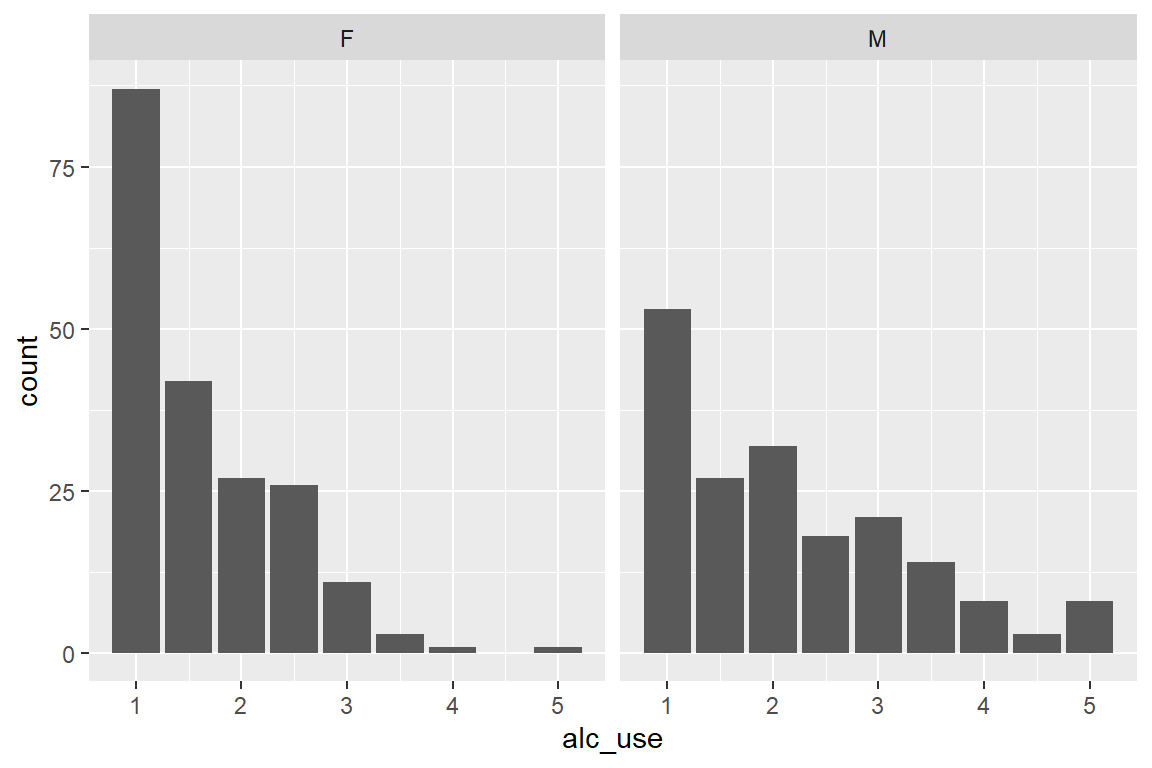
\includegraphics{chapter4_files/figure-latex/unnamed-chunk-9-1.pdf}

All the variables after scaling had a mean of 0 and most of variables'
values ranged from -4 and 4, only except for variables crim (crime
rate), which might be due to out-liers (corresponds to the finding from
the correlation matrix).\\
\#\# 4.3 Use the quantiles as the break points in the categorical
variable and drop the old crime rate variable from the dataset.

\begin{Shaded}
\begin{Highlighting}[]
\CommentTok{\#generate cutoff according to quantile}
\NormalTok{bins }\OtherTok{\textless{}{-}} \FunctionTok{quantile}\NormalTok{(bos.s}\SpecialCharTok{$}\NormalTok{crim)}
\CommentTok{\#generate a categorical variable "crime" and re{-}code it}
\NormalTok{bos.s }\OtherTok{\textless{}{-}}\NormalTok{ bos.s }\SpecialCharTok{\%\textgreater{}\%} 
  \FunctionTok{mutate}\NormalTok{(}\AttributeTok{crime =}\NormalTok{ crim }\SpecialCharTok{\%\textgreater{}\%} 
           \FunctionTok{cut}\NormalTok{(}\AttributeTok{breaks =}\NormalTok{ bins, }\AttributeTok{include.lowest =} \ConstantTok{TRUE}\NormalTok{) }\SpecialCharTok{\%\textgreater{}\%} 
           \FunctionTok{fct\_recode}\NormalTok{(}\StringTok{"Low"} \OtherTok{=} \StringTok{"[{-}0.419,{-}0.411]"}\NormalTok{,}
                     \StringTok{"MediumLow"} \OtherTok{=} \StringTok{"({-}0.411,{-}0.39]"}\NormalTok{,}
                     \StringTok{"MediumHigh"} \OtherTok{=} \StringTok{"({-}0.39,0.00739]"}\NormalTok{,}
                     \StringTok{"High"} \OtherTok{=} \StringTok{"(0.00739,9.92]"}\NormalTok{))}
\CommentTok{\#remove crim}
\NormalTok{bos.s }\OtherTok{\textless{}{-}}\NormalTok{ bos.s }\SpecialCharTok{\%\textgreater{}\%} \FunctionTok{select}\NormalTok{(}\SpecialCharTok{{-}}\NormalTok{crim)}
\end{Highlighting}
\end{Shaded}

\hypertarget{divide-the-dataset-to-train-and-test-sets-so-that-80-of-the-data-belongs-to-the-train-set}{%
\subsection{4.4 Divide the dataset to train and test sets, so that 80\%
of the data belongs to the train
set}\label{divide-the-dataset-to-train-and-test-sets-so-that-80-of-the-data-belongs-to-the-train-set}}

\begin{Shaded}
\begin{Highlighting}[]
\FunctionTok{set.seed}\NormalTok{(}\DecValTok{2022}\NormalTok{) }
\CommentTok{\#generate an object containing the number of observations in bos dataset}
\NormalTok{n }\OtherTok{\textless{}{-}}  \FunctionTok{nrow}\NormalTok{(bos.s)}

\CommentTok{\#generate an object "ind", which contains a random selected set of the indexing }
\CommentTok{\#of bos dataset, and the number of indexing takes up 80\% of number of observations}
\NormalTok{ind }\OtherTok{\textless{}{-}} \FunctionTok{sample}\NormalTok{(}\DecValTok{1}\SpecialCharTok{:}\NormalTok{n, }\AttributeTok{size =}\NormalTok{ n}\SpecialCharTok{*}\FloatTok{0.8}\NormalTok{)}
\CommentTok{\#generate train\&test sets according to the random set of indexing number}
\NormalTok{train }\OtherTok{\textless{}{-}}\NormalTok{ bos.s[ind,]}
\NormalTok{test }\OtherTok{\textless{}{-}}\NormalTok{ bos.s[}\SpecialCharTok{{-}}\NormalTok{ind,]}
\end{Highlighting}
\end{Shaded}

\hypertarget{fit-the-linear-discriminant-analysis-on-the-train-set.-use-the-categorical-crime-rate-as-the-target-variable-and-all-the-other-variables-in-the-dataset-as-predictor-variables.-draw-the-lda-biplot-0-3-points}{%
\subsection{5 Fit the linear discriminant analysis on the train set. Use
the categorical crime rate as the target variable and all the other
variables in the dataset as predictor variables. Draw the LDA (bi)plot
(0-3
points)}\label{fit-the-linear-discriminant-analysis-on-the-train-set.-use-the-categorical-crime-rate-as-the-target-variable-and-all-the-other-variables-in-the-dataset-as-predictor-variables.-draw-the-lda-biplot-0-3-points}}

\hypertarget{fit-the-linear-discriminant-analysis-on-the-train-set-use-the-categorical-crime-rate-as-the-target-variable-and-all-the-other-variables-in-the-dataset-as-predictor-variables}{%
\subsubsection{5.1 Fit the linear discriminant analysis on the train set
(Use the categorical crime rate as the target variable and all the other
variables in the dataset as predictor
variables)}\label{fit-the-linear-discriminant-analysis-on-the-train-set-use-the-categorical-crime-rate-as-the-target-variable-and-all-the-other-variables-in-the-dataset-as-predictor-variables}}

\begin{Shaded}
\begin{Highlighting}[]
\CommentTok{\# fit an linear discriminant model on the train set, named as "lda.fit"}
\NormalTok{lda.fit }\OtherTok{\textless{}{-}} \FunctionTok{lda}\NormalTok{(crime }\SpecialCharTok{\textasciitilde{}}\NormalTok{ ., }\AttributeTok{data =}\NormalTok{ train) }
\end{Highlighting}
\end{Shaded}

\hypertarget{draw-the-lda-biplot}{%
\subsubsection{5.2 Draw the LDA (bi)plot}\label{draw-the-lda-biplot}}

\begin{Shaded}
\begin{Highlighting}[]
\CommentTok{\# the function for lda biplot arrows}
\NormalTok{lda.arrows }\OtherTok{\textless{}{-}} \ControlFlowTok{function}\NormalTok{(x, }\AttributeTok{myscale =} \DecValTok{1}\NormalTok{, }\AttributeTok{arrow\_heads =} \FloatTok{0.1}\NormalTok{, }\AttributeTok{color =} \StringTok{"red"}\NormalTok{, }\AttributeTok{tex =} \FloatTok{0.75}\NormalTok{, }\AttributeTok{choices =} \FunctionTok{c}\NormalTok{(}\DecValTok{1}\NormalTok{,}\DecValTok{2}\NormalTok{))\{}
\NormalTok{  heads }\OtherTok{\textless{}{-}} \FunctionTok{coef}\NormalTok{(x)}
  \FunctionTok{arrows}\NormalTok{(}\AttributeTok{x0 =} \DecValTok{0}\NormalTok{, }\AttributeTok{y0 =} \DecValTok{0}\NormalTok{, }
         \AttributeTok{x1 =}\NormalTok{ myscale }\SpecialCharTok{*}\NormalTok{ heads[,choices[}\DecValTok{1}\NormalTok{]], }
         \AttributeTok{y1 =}\NormalTok{ myscale }\SpecialCharTok{*}\NormalTok{ heads[,choices[}\DecValTok{2}\NormalTok{]], }\AttributeTok{col=}\NormalTok{color, }\AttributeTok{length =}\NormalTok{ arrow\_heads)}
  \FunctionTok{text}\NormalTok{(myscale }\SpecialCharTok{*}\NormalTok{ heads[,choices], }\AttributeTok{labels =} \FunctionTok{row.names}\NormalTok{(heads), }
       \AttributeTok{cex =}\NormalTok{ tex, }\AttributeTok{col=}\NormalTok{color, }\AttributeTok{pos=}\DecValTok{3}\NormalTok{)}
\NormalTok{\}}
\CommentTok{\# target classes as numeric}
\NormalTok{classes }\OtherTok{\textless{}{-}} \FunctionTok{as.numeric}\NormalTok{(}\FunctionTok{factor}\NormalTok{(train}\SpecialCharTok{$}\NormalTok{crime))}
\end{Highlighting}
\end{Shaded}

\begin{Shaded}
\begin{Highlighting}[]
\CommentTok{\#plot the lda results}
\FunctionTok{plot}\NormalTok{(lda.fit, }\AttributeTok{dimen =} \DecValTok{2}\NormalTok{,  }\AttributeTok{pch =}\NormalTok{ classes, }\AttributeTok{col =}\NormalTok{ classes)}\SpecialCharTok{+}
\FunctionTok{lda.arrows}\NormalTok{(lda.fit, }\AttributeTok{myscale =} \DecValTok{4}\NormalTok{)}
\end{Highlighting}
\end{Shaded}

\begin{figure}
\centering
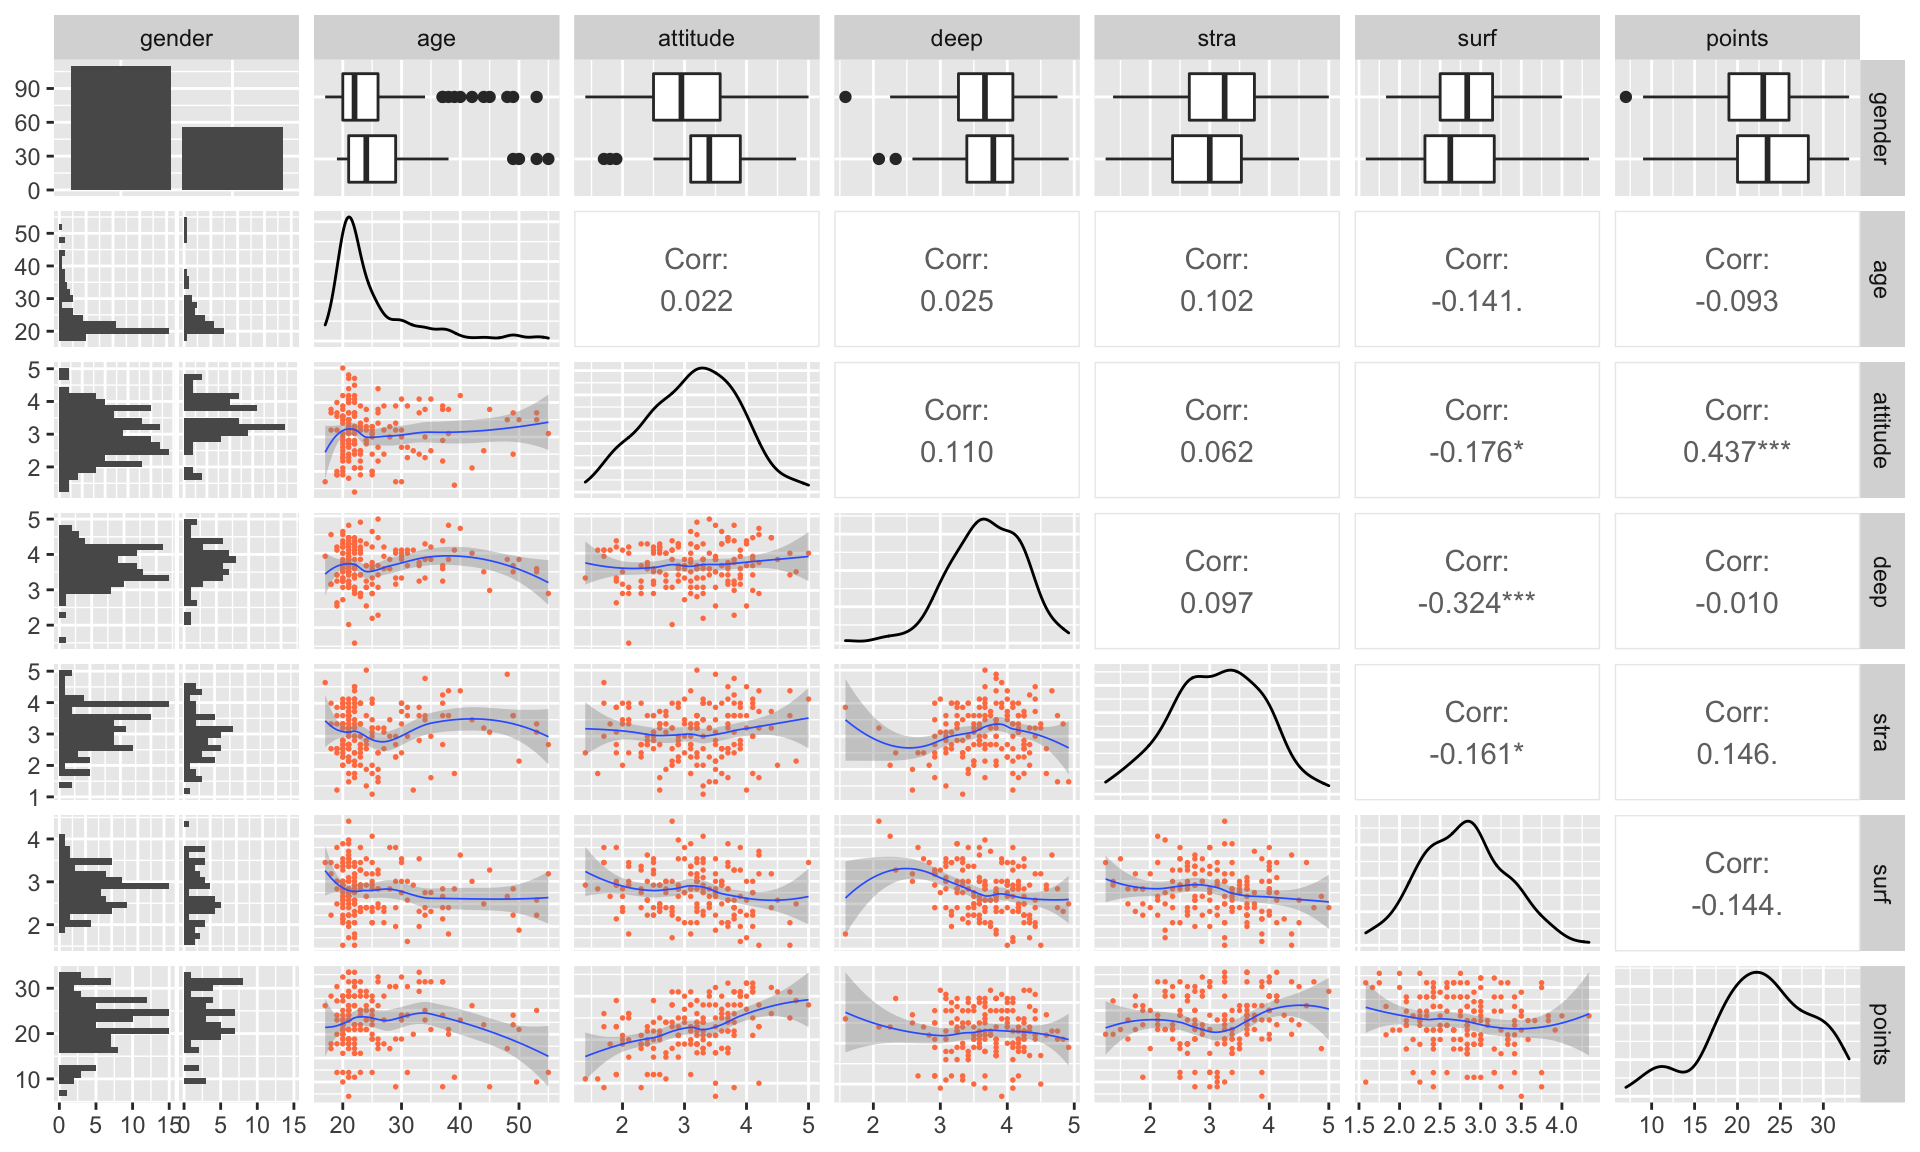
\includegraphics{chapter4_files/figure-latex/unnamed-chunk-14-1.pdf}
\caption{Fig 5.2 Biplot for LDA for clustering crime rate}
\end{figure}

\begin{verbatim}
## integer(0)
\end{verbatim}

Biplot based on LD1 and LD2 was generated, see fig 5.2. The most of four
clusters separated poorly, except for the cluster ``High''. Heavy
overlap was observed between each pair of other cluster. Besides,
Clusters High and MediumHigh also showed notable overlaps.

Based on arrows, varaibles lstat explained the most for cluster High.
Contributions of variables to other clusters are not clear enough due to
the heavy overlap.

\hypertarget{save-the-crime-categories-from-the-test-set-and-then-remove-the-categorical-crime-variable-from-the-test-dataset.-then-predict-the-classes-with-the-lda-model-on-the-test-data.-cross-tabulate-the-results-with-the-crime-categories-from-the-test-set.-comment-on-the-results.-0-3-points}{%
\subsection{6 Save the crime categories from the test set and then
remove the categorical crime variable from the test dataset. Then
predict the classes with the LDA model on the test data. Cross tabulate
the results with the crime categories from the test set. Comment on the
results. (0-3
points)}\label{save-the-crime-categories-from-the-test-set-and-then-remove-the-categorical-crime-variable-from-the-test-dataset.-then-predict-the-classes-with-the-lda-model-on-the-test-data.-cross-tabulate-the-results-with-the-crime-categories-from-the-test-set.-comment-on-the-results.-0-3-points}}

\hypertarget{save-the-crime-categories-from-the-test-set-and-then-remove-the-categorical-crime-variable-from-the-test-dataset}{%
\subsubsection{6.1 Save the crime categories from the test set and then
remove the categorical crime variable from the test
dataset}\label{save-the-crime-categories-from-the-test-set-and-then-remove-the-categorical-crime-variable-from-the-test-dataset}}

\begin{Shaded}
\begin{Highlighting}[]
\CommentTok{\#save crime into an object}
\NormalTok{classes.test }\OtherTok{\textless{}{-}}\NormalTok{ test}\SpecialCharTok{$}\NormalTok{crime}
\CommentTok{\#remove crime}
\NormalTok{test}\SpecialCharTok{$}\NormalTok{crime }\OtherTok{\textless{}{-}} \ConstantTok{NULL}
\end{Highlighting}
\end{Shaded}

\hypertarget{predict-the-classes-with-the-lda-model-on-the-test-data}{%
\subsubsection{6.2 predict the classes with the LDA model on the test
data}\label{predict-the-classes-with-the-lda-model-on-the-test-data}}

\begin{Shaded}
\begin{Highlighting}[]
\NormalTok{predicted.test }\OtherTok{\textless{}{-}} \FunctionTok{predict}\NormalTok{(lda.fit, test)}
\end{Highlighting}
\end{Shaded}

\hypertarget{cross-tabulate-the-results-with-the-crime-categories-from-the-test-set.}{%
\subsubsection{6.3 Cross tabulate the results with the crime categories
from the test
set.}\label{cross-tabulate-the-results-with-the-crime-categories-from-the-test-set.}}

\begin{Shaded}
\begin{Highlighting}[]
\CommentTok{\#generate a table that evaluate the accuracy of model, and pass the table into}
\CommentTok{\#an object named "accuracy.tab"}
\NormalTok{accuracy.tab }\OtherTok{\textless{}{-}} \FunctionTok{table}\NormalTok{(}\AttributeTok{correct =}\NormalTok{ classes.test, }\AttributeTok{predicted =}\NormalTok{ predicted.test}\SpecialCharTok{$}\NormalTok{class )}

\CommentTok{\#show the accuracy table}
\NormalTok{accuracy.tab}
\end{Highlighting}
\end{Shaded}

\begin{verbatim}
##             predicted
## correct      Low MediumLow MediumHigh High
##   Low          4         7          0    0
##   MediumLow   10        16          4    0
##   MediumHigh   2        11         17    1
##   High         0         0          0   30
\end{verbatim}

\begin{Shaded}
\begin{Highlighting}[]
\CommentTok{\#ask R to identify the correct predictions and add them up}
\NormalTok{correct.n }\OtherTok{=} \DecValTok{0} \CommentTok{\# the number of correct predictions starting at 0}
\ControlFlowTok{for}\NormalTok{ (i }\ControlFlowTok{in} \DecValTok{1}\SpecialCharTok{:}\DecValTok{4}\NormalTok{)\{ }\CommentTok{\#4 loops because we have 4 rows/columns}
\NormalTok{  correct.c }\OtherTok{\textless{}{-}}\NormalTok{ accuracy.tab[}
    \FunctionTok{which}\NormalTok{(}\FunctionTok{rownames}\NormalTok{(accuracy.tab) }\SpecialCharTok{==} \FunctionTok{colnames}\NormalTok{(accuracy.tab)[i]), }
\NormalTok{    i] }\CommentTok{\# if a cell has same row and column names, pass its value into "correct.c"}
\NormalTok{  correct.n }\OtherTok{=}\NormalTok{ correct.c}\SpecialCharTok{+}\NormalTok{ correct.n }\CommentTok{\# update the value of correct prediction}
\NormalTok{\}                                  }\CommentTok{\# by adding "correct.c"}

\CommentTok{\# calculate the percent of correct predictions for test set}
\NormalTok{correct.n}\SpecialCharTok{/}\NormalTok{(}\FunctionTok{nrow}\NormalTok{(bos.s)}\SpecialCharTok{*}\FloatTok{0.2}\NormalTok{) }\CommentTok{\#denominator is the number of obs. in test set}
\end{Highlighting}
\end{Shaded}

\begin{verbatim}
## [1] 0.6620553
\end{verbatim}

\hypertarget{comment-on-the-results}{%
\subsubsection{6.4 Comment on the
results}\label{comment-on-the-results}}

Overall, 66.2\% of the predictions are correct, showing not quite
satisfactory predicting effect of our linear discriminant analysis.
Observe the result closely, it is found that the for high and medium
high crime rate regions, the analysis did the best predictions, with
90\% (47/52) of accuracy. For Low and medium low regions, the predictive
effect of our analysis decreased tremendously. This might be the result
of \emph{a.} the violation of the assumption of multivariate normality
(but evidence showed even when this is violated, LDA also exhibited good
accuracy); \emph{b.} large number of out-liers in the dependent variable
before re-coding (LDA is sensitive to out-liers); \emph{c.} The small
size of category Low in test set; \emph{d.} better categorization
strategy for dependent variable needed (the current categorization is
only base on quantiles, which is lack of more evidence-based
foundation).

\hypertarget{reload-the-boston-dataset-and-standardize-the-dataset-we-did-not-do-this-in-the-exercise-set-but-you-should-scale-the-variables-to-get-comparable-distances.-calculate-the-distances-between-the-observations.-run-k-means-algorithm-on-the-dataset.-investigate-what-is-the-optimal-number-of-clusters-and-run-the-algorithm-again.-visualize-the-clusters-for-example-with-the-pairs-or-ggpairs-functions-where-the-clusters-are-separated-with-colors-and-interpret-the-results.-0-4-points}{%
\subsection{7 Reload the Boston dataset and standardize the dataset (we
did not do this in the Exercise Set, but you should scale the variables
to get comparable distances). Calculate the distances between the
observations. Run k-means algorithm on the dataset. Investigate what is
the optimal number of clusters and run the algorithm again. Visualize
the clusters (for example with the pairs() or ggpairs() functions, where
the clusters are separated with colors) and interpret the results. (0-4
points)}\label{reload-the-boston-dataset-and-standardize-the-dataset-we-did-not-do-this-in-the-exercise-set-but-you-should-scale-the-variables-to-get-comparable-distances.-calculate-the-distances-between-the-observations.-run-k-means-algorithm-on-the-dataset.-investigate-what-is-the-optimal-number-of-clusters-and-run-the-algorithm-again.-visualize-the-clusters-for-example-with-the-pairs-or-ggpairs-functions-where-the-clusters-are-separated-with-colors-and-interpret-the-results.-0-4-points}}

\hypertarget{reload-the-boston-dataset-and-standardize-the-dataset}{%
\subsubsection{7.1 Reload the Boston dataset and standardize the
dataset}\label{reload-the-boston-dataset-and-standardize-the-dataset}}

\begin{Shaded}
\begin{Highlighting}[]
\CommentTok{\#reload Boston}
\FunctionTok{data}\NormalTok{(}\StringTok{"Boston"}\NormalTok{)}
\NormalTok{bos }\OtherTok{\textless{}{-}}\NormalTok{ Boston}
\CommentTok{\#standardize the dataset}
\NormalTok{bos.s }\OtherTok{\textless{}{-}} \FunctionTok{as.data.frame}\NormalTok{(}\FunctionTok{scale}\NormalTok{(bos))}
\end{Highlighting}
\end{Shaded}

\hypertarget{calculate-the-distances-between-the-observations}{%
\subsubsection{7.2 Calculate the distances between the
observations}\label{calculate-the-distances-between-the-observations}}

\begin{Shaded}
\begin{Highlighting}[]
\NormalTok{dis\_eu }\OtherTok{\textless{}{-}} \FunctionTok{dist}\NormalTok{(bos.s)}
\FunctionTok{summary}\NormalTok{(dis\_eu)}
\end{Highlighting}
\end{Shaded}

\begin{verbatim}
##    Min. 1st Qu.  Median    Mean 3rd Qu.    Max. 
##  0.1343  3.4625  4.8241  4.9111  6.1863 14.3970
\end{verbatim}

\hypertarget{run-k-means-algorithm-on-the-dataset}{%
\subsubsection{7.3 Run k-means algorithm on the
dataset}\label{run-k-means-algorithm-on-the-dataset}}

\begin{Shaded}
\begin{Highlighting}[]
\NormalTok{bos.s.km }\OtherTok{\textless{}{-}} \FunctionTok{kmeans}\NormalTok{(bos.s, }\AttributeTok{centers =} \DecValTok{4}\NormalTok{) }
\end{Highlighting}
\end{Shaded}

\hypertarget{investigate-what-is-the-optimal-number-of-clusters}{%
\subsubsection{7.4 Investigate what is the optimal number of
clusters}\label{investigate-what-is-the-optimal-number-of-clusters}}

\begin{Shaded}
\begin{Highlighting}[]
\FunctionTok{date}\NormalTok{()}
\end{Highlighting}
\end{Shaded}

\begin{verbatim}
## [1] "Tue Nov 22 22:04:38 2022"
\end{verbatim}

\begin{Shaded}
\begin{Highlighting}[]
\FunctionTok{set.seed}\NormalTok{(}\DecValTok{22}\NormalTok{) }\CommentTok{\#22 is the date I carried out the analysis}

\CommentTok{\# determine the number of clusters}
\NormalTok{k\_max }\OtherTok{\textless{}{-}} \DecValTok{10}

\CommentTok{\# calculate the total within sum of squares}
\NormalTok{twcss }\OtherTok{\textless{}{-}} \FunctionTok{sapply}\NormalTok{(}\DecValTok{1}\SpecialCharTok{:}\NormalTok{k\_max, }\ControlFlowTok{function}\NormalTok{(k)\{}\FunctionTok{kmeans}\NormalTok{(bos.s, k)}\SpecialCharTok{$}\NormalTok{tot.withinss\})}
\end{Highlighting}
\end{Shaded}

\begin{Shaded}
\begin{Highlighting}[]
\CommentTok{\# visualize the results}
\FunctionTok{qplot}\NormalTok{(}\AttributeTok{x =} \DecValTok{1}\SpecialCharTok{:}\NormalTok{k\_max, }\AttributeTok{y =}\NormalTok{ twcss, }\AttributeTok{geom =} \StringTok{\textquotesingle{}line\textquotesingle{}}\NormalTok{)}\SpecialCharTok{+}
  \FunctionTok{geom\_line}\NormalTok{(}\FunctionTok{aes}\NormalTok{(}\AttributeTok{x =} \DecValTok{3}\NormalTok{, }\AttributeTok{color =} \StringTok{"red"}\NormalTok{)) }\SpecialCharTok{+}
  \FunctionTok{annotate}\NormalTok{(}\StringTok{"text"}\NormalTok{, }
           \AttributeTok{label =} 
             \StringTok{"←Elbow effect happens here"}\NormalTok{, }
           \AttributeTok{x =} \FloatTok{4.8}\NormalTok{, }\AttributeTok{y =}\DecValTok{3800}\NormalTok{, }\AttributeTok{color =} \StringTok{"red"}\NormalTok{) }
\end{Highlighting}
\end{Shaded}

\begin{verbatim}
## Warning in grid.Call.graphics(C_text, as.graphicsAnnot(x$label), x$x, x$y, :
## 'mbcsToSbcs'里转换'←Elbow effect happens here'出错:<e2>代替了dot
\end{verbatim}

\begin{verbatim}
## Warning in grid.Call.graphics(C_text, as.graphicsAnnot(x$label), x$x, x$y, :
## 'mbcsToSbcs'里转换'←Elbow effect happens here'出错:<86>代替了dot
\end{verbatim}

\begin{verbatim}
## Warning in grid.Call.graphics(C_text, as.graphicsAnnot(x$label), x$x, x$y, :
## 'mbcsToSbcs'里转换'←Elbow effect happens here'出错:<90>代替了dot
\end{verbatim}

\begin{figure}
\centering
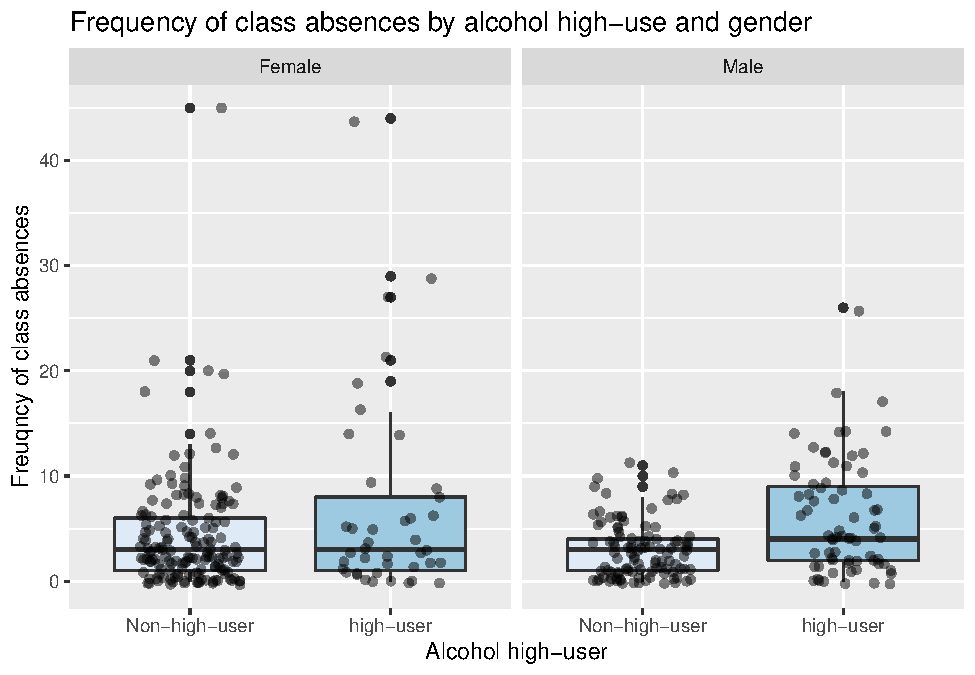
\includegraphics{chapter4_files/figure-latex/unnamed-chunk-22-1.pdf}
\caption{Fig 7.4 Elbow plot for trends of within-cluster sum-of-square
with increasing number of k}
\end{figure}

There is a huge reduction in variation with K =3, but after that the
variation does not go down as quickly. I will use K = 3 and do the
k-means clustering again.

\hypertarget{run-the-algorithm-again}{%
\subsubsection{7.5 run the algorithm
again}\label{run-the-algorithm-again}}

\begin{Shaded}
\begin{Highlighting}[]
\NormalTok{km }\OtherTok{\textless{}{-}} \FunctionTok{kmeans}\NormalTok{(bos.s, }\AttributeTok{centers =} \DecValTok{3}\NormalTok{)}
\end{Highlighting}
\end{Shaded}

\hypertarget{visualize-the-clusters}{%
\subsubsection{7.6 Visualize the
clusters}\label{visualize-the-clusters}}

\begin{Shaded}
\begin{Highlighting}[]
\CommentTok{\#define a function that allows me to fine{-}tune the matrix}
\NormalTok{my.fun.km }\OtherTok{\textless{}{-}} \ControlFlowTok{function}\NormalTok{(data, mapping,...)\{ }\CommentTok{\#define arguments}
\NormalTok{  p }\OtherTok{\textless{}{-}} \FunctionTok{ggplot}\NormalTok{(}\AttributeTok{data =}\NormalTok{ data, }\AttributeTok{mapping =}\NormalTok{ mapping) }\SpecialCharTok{+} \CommentTok{\#pass arguments}
    \FunctionTok{geom\_point}\NormalTok{(}\AttributeTok{size =} \FloatTok{0.3}\NormalTok{, }
               \AttributeTok{color =} \FunctionTok{factor}\NormalTok{(km}\SpecialCharTok{$}\NormalTok{cluster),}
\NormalTok{               ...) }\SpecialCharTok{+} \CommentTok{\#define points size and color}
    \FunctionTok{stat\_ellipse}\NormalTok{(}\AttributeTok{geom =} \StringTok{"polygon"}\NormalTok{, }\AttributeTok{mapping =}\NormalTok{ mapping, }\AttributeTok{alpha =} \FloatTok{0.5}\NormalTok{)}
     \CommentTok{\#calculate an ellipse layer that separate clusters}
\NormalTok{  p }\CommentTok{\#print the results}
\NormalTok{\}}

\FunctionTok{ggpairs}\NormalTok{(bos, }\AttributeTok{mapping =} \FunctionTok{aes}\NormalTok{(}\AttributeTok{fill=}\FunctionTok{factor}\NormalTok{(km}\SpecialCharTok{$}\NormalTok{cluster)),}
        \AttributeTok{lower =} \FunctionTok{list}\NormalTok{(}
          \AttributeTok{continuous =}\NormalTok{ my.fun.km}
\NormalTok{          ),}
        \AttributeTok{col =} \DecValTok{1}\SpecialCharTok{:}\DecValTok{7}\NormalTok{)}
\end{Highlighting}
\end{Shaded}

\begin{figure}
\centering
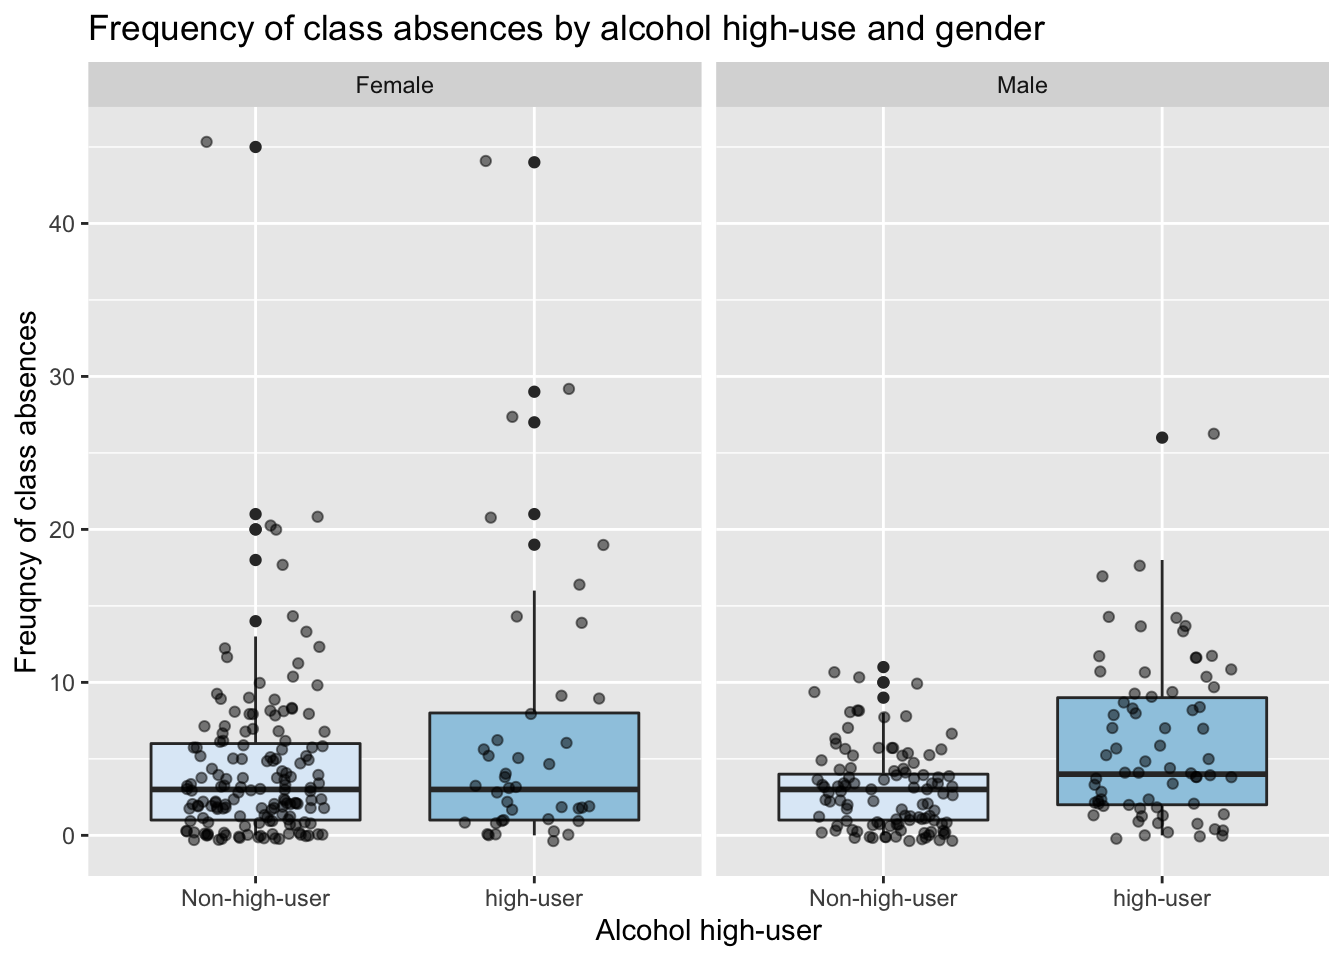
\includegraphics{chapter4_files/figure-latex/unnamed-chunk-24-1.pdf}
\caption{Fig 7.6.1 Correlation Matrix with clusters}
\end{figure}

\begin{Shaded}
\begin{Highlighting}[]
\FunctionTok{ggpairs}\NormalTok{(bos, }\AttributeTok{mapping =} \FunctionTok{aes}\NormalTok{(}\AttributeTok{fill=}\FunctionTok{factor}\NormalTok{(km}\SpecialCharTok{$}\NormalTok{cluster)),}
        \AttributeTok{lower =} \FunctionTok{list}\NormalTok{(}
          \AttributeTok{continuous =}\NormalTok{ my.fun.km}
\NormalTok{          ),}
        \AttributeTok{col =} \DecValTok{8}\SpecialCharTok{:}\DecValTok{14}\NormalTok{) }
\end{Highlighting}
\end{Shaded}

\begin{figure}
\centering
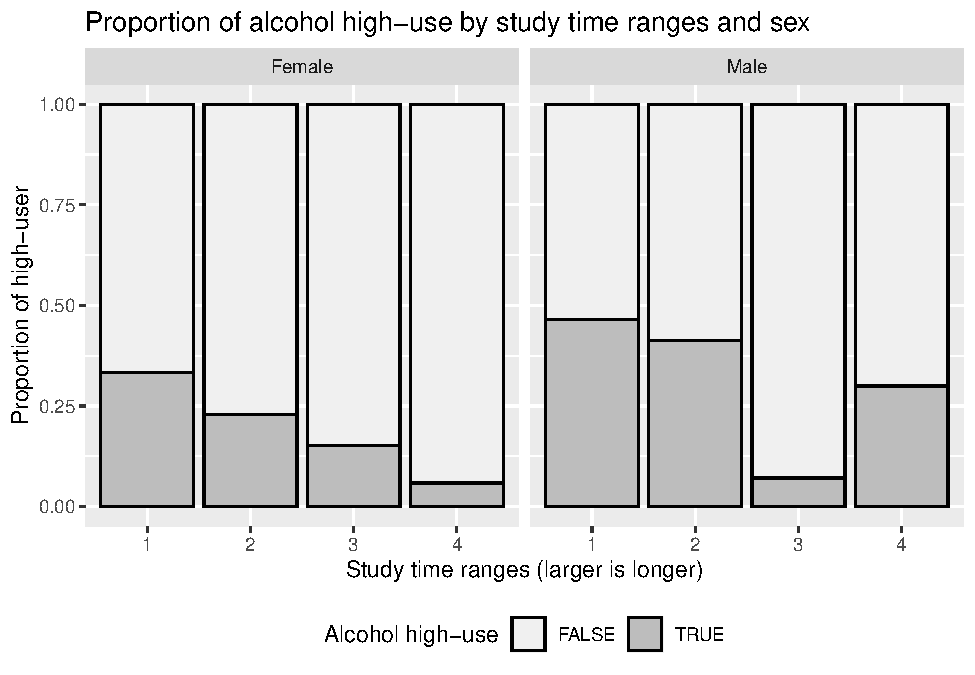
\includegraphics{chapter4_files/figure-latex/unnamed-chunk-25-1.pdf}
\caption{Fig 7.6.2 Correlation Matrix with clusters}
\end{figure}

\hypertarget{interpret-the-results}{%
\subsubsection{7.7 interpret the results}\label{interpret-the-results}}

By observing the elbow plot that depicts the how size of within-cluster
sum-of-square changes with number of k, an optimal number of k = 3 was
determined. The subsequent results of k-means clustering was visualized
in a correlation matrix with containing variables in dataset. It is
observed that some of the variables have contributed tremendously to the
clustering. For example, the variable black separates 1 cluster with the
other 2 clusters nicely, see the 5th column of the picture above (Fig
7.6.2), x axis; and the variable age separates a different cluster with
the other 2 clusters roughly, see the 7th row of the picture above (Fig
7.6.1), y axis. Some pairs of the variables have also played important
role in clustering, for example, the combination of black and dist
variables separate the 3 clusters roughly, see picture above (Fig 7.6.2,
column 1nd, row 5th) or see the picture below (Fig 7.6.3). Due to the
limitation of presenting more dimensions in a 2-dimension screen, I am
not able to dig into the clustering effect of more variables combined.
Fortunately, k-means clustering has done that for me, mathematically.

\begin{Shaded}
\begin{Highlighting}[]
\NormalTok{bos }\SpecialCharTok{\%\textgreater{}\%} \FunctionTok{ggplot}\NormalTok{(}\FunctionTok{aes}\NormalTok{(}\AttributeTok{x =}\NormalTok{ dis, }\AttributeTok{y =}\NormalTok{ black, }\AttributeTok{color =} \FunctionTok{factor}\NormalTok{(km}\SpecialCharTok{$}\NormalTok{cluster))) }\SpecialCharTok{+}
  \FunctionTok{geom\_point}\NormalTok{() }\SpecialCharTok{+}
  \FunctionTok{geom\_abline}\NormalTok{(}\AttributeTok{intercept =} \DecValTok{480}\NormalTok{, }\AttributeTok{slope =} \SpecialCharTok{{-}}\DecValTok{25}\NormalTok{)}\SpecialCharTok{+}
  \FunctionTok{geom\_abline}\NormalTok{(}\AttributeTok{intercept =} \DecValTok{400}\NormalTok{, }\AttributeTok{slope =} \SpecialCharTok{{-}}\DecValTok{80}\NormalTok{) }\SpecialCharTok{+}
  \FunctionTok{stat\_ellipse}\NormalTok{(}\AttributeTok{geom =} \StringTok{"polygon"}\NormalTok{,}
               \FunctionTok{aes}\NormalTok{(}\AttributeTok{fill =}\NormalTok{ km}\SpecialCharTok{$}\NormalTok{cluster),}
               \AttributeTok{alpha =} \FloatTok{0.25}\NormalTok{)}
\end{Highlighting}
\end{Shaded}

\begin{figure}
\centering
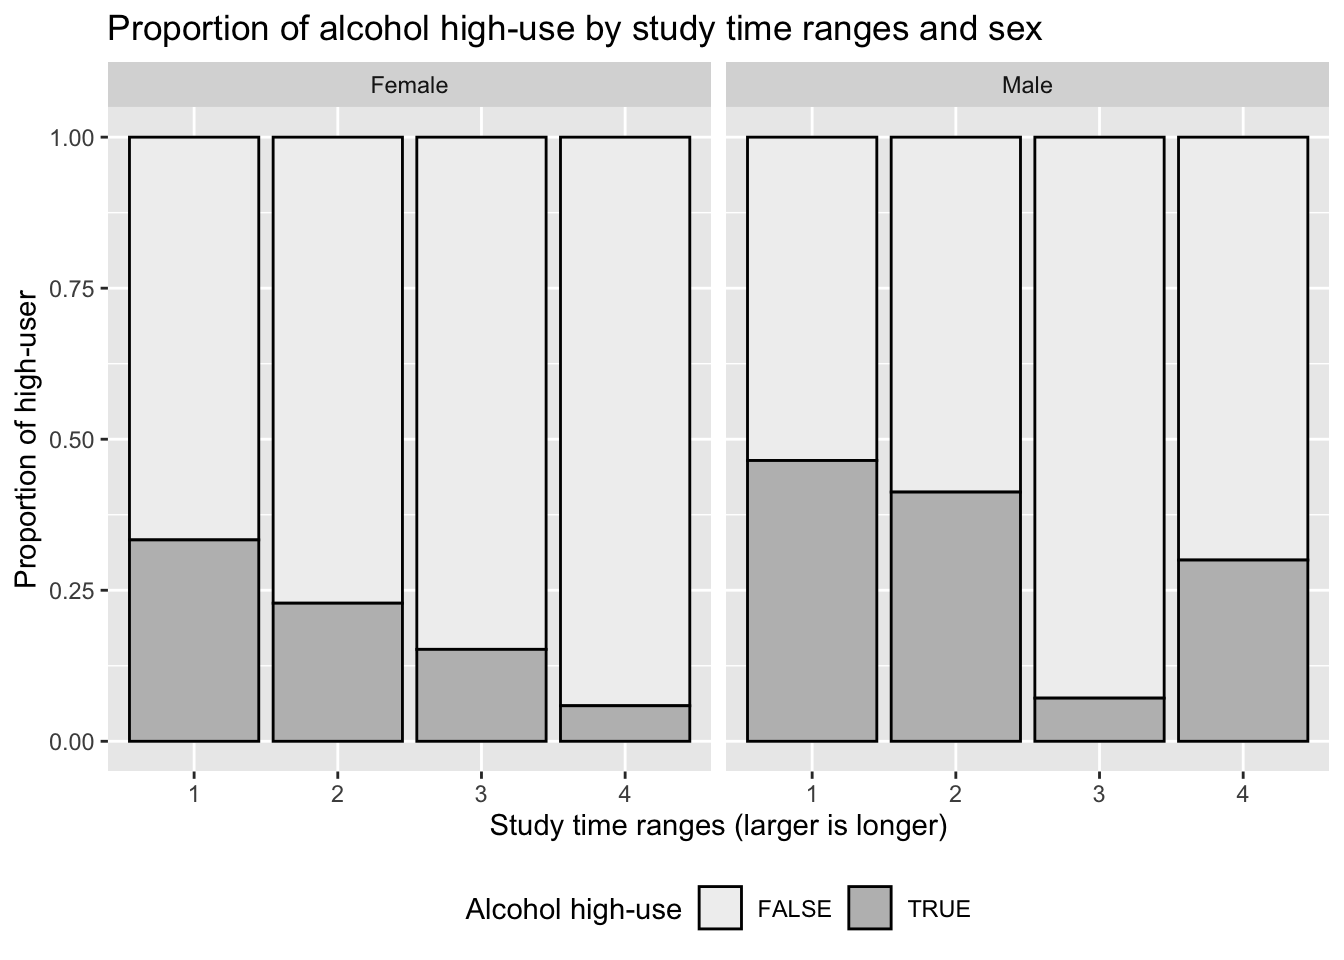
\includegraphics{chapter4_files/figure-latex/unnamed-chunk-26-1.pdf}
\caption{the clustering effect of variables black and dis combined}
\end{figure}

\hypertarget{bonus-perform-k-means-on-the-original-boston-data-with-some-reasonable-number-of-clusters-2.-remember-to-standardize-the-dataset.-then-perform-lda-using-the-clusters-as-target-classes.-include-all-the-variables-in-the-boston-data-in-the-lda-model.-visualize-the-results-with-a-biplot-include-arrows-representing-the-relationships-of-the-original-variables-to-the-lda-solution.-interpret-the-results.-which-variables-are-the-most-influential-linear-separators-for-the-clusters-0-2-points-to-compensate-any-loss-of-points-from-the-above-exercises}{%
\subsection{8 Bonus: Perform k-means on the original Boston data with
some reasonable number of clusters (\textgreater{} 2). Remember to
standardize the dataset. Then perform LDA using the clusters as target
classes. Include all the variables in the Boston data in the LDA model.
Visualize the results with a biplot (include arrows representing the
relationships of the original variables to the LDA solution). Interpret
the results. Which variables are the most influential linear separators
for the clusters? (0-2 points to compensate any loss of points from the
above
exercises)}\label{bonus-perform-k-means-on-the-original-boston-data-with-some-reasonable-number-of-clusters-2.-remember-to-standardize-the-dataset.-then-perform-lda-using-the-clusters-as-target-classes.-include-all-the-variables-in-the-boston-data-in-the-lda-model.-visualize-the-results-with-a-biplot-include-arrows-representing-the-relationships-of-the-original-variables-to-the-lda-solution.-interpret-the-results.-which-variables-are-the-most-influential-linear-separators-for-the-clusters-0-2-points-to-compensate-any-loss-of-points-from-the-above-exercises}}

\hypertarget{perform-k-means-on-the-original-boston-data-with-some-reasonable-number-of-clusters-2remember-to-standardize-the-dataset}{%
\subsubsection{8.1 Perform k-means on the original Boston data with some
reasonable number of clusters (\textgreater{} 2)(Remember to standardize
the
dataset)}\label{perform-k-means-on-the-original-boston-data-with-some-reasonable-number-of-clusters-2remember-to-standardize-the-dataset}}

\begin{Shaded}
\begin{Highlighting}[]
\CommentTok{\# k = 3 is the optimal clusters found}
\NormalTok{km }\OtherTok{\textless{}{-}} \FunctionTok{kmeans}\NormalTok{(}\FunctionTok{scale}\NormalTok{(Boston), }\AttributeTok{centers =} \DecValTok{3}\NormalTok{)}
\end{Highlighting}
\end{Shaded}

\hypertarget{perform-lda-using-the-clusters-as-target-classes.}{%
\subsubsection{8.2 Perform LDA using the clusters as target
classes.}\label{perform-lda-using-the-clusters-as-target-classes.}}

\begin{Shaded}
\begin{Highlighting}[]
\CommentTok{\#reload and standardize data}
\NormalTok{bos.s  }\OtherTok{\textless{}{-}} \FunctionTok{as.data.frame}\NormalTok{(}\FunctionTok{scale}\NormalTok{(Boston))}
\CommentTok{\#save the clusters identified by k{-}means clustering as a column in the data set}
\NormalTok{bos.s}\SpecialCharTok{$}\NormalTok{km.cluster }\OtherTok{\textless{}{-}}\NormalTok{ km}\SpecialCharTok{$}\NormalTok{cluster}
\NormalTok{lda.km }\OtherTok{\textless{}{-}} \FunctionTok{lda}\NormalTok{(km.cluster }\SpecialCharTok{\textasciitilde{}}\NormalTok{ ., }\AttributeTok{data =}\NormalTok{ bos.s) }
\end{Highlighting}
\end{Shaded}

\hypertarget{visualize-the-results-with-a-biplot-include-arrows-representing-the-relationships-of-the-original-variables-to-the-lda-solution}{%
\subsubsection{8.3 Visualize the results with a biplot (include arrows
representing the relationships of the original variables to the LDA
solution)}\label{visualize-the-results-with-a-biplot-include-arrows-representing-the-relationships-of-the-original-variables-to-the-lda-solution}}

\begin{Shaded}
\begin{Highlighting}[]
\CommentTok{\# target classes as numeric}
\NormalTok{classes }\OtherTok{\textless{}{-}} \FunctionTok{as.numeric}\NormalTok{(}\FunctionTok{factor}\NormalTok{(bos.s}\SpecialCharTok{$}\NormalTok{km.cluster))}
\CommentTok{\#plot the lda results as biplot}
\FunctionTok{plot}\NormalTok{(lda.km, }\AttributeTok{dimen =} \DecValTok{2}\NormalTok{,  }\AttributeTok{pch =}\NormalTok{ classes, }\AttributeTok{col =}\NormalTok{ classes)}\SpecialCharTok{+}
\FunctionTok{lda.arrows}\NormalTok{(lda.km, }\AttributeTok{myscale =} \DecValTok{4}\NormalTok{)}
\end{Highlighting}
\end{Shaded}

\begin{figure}
\centering
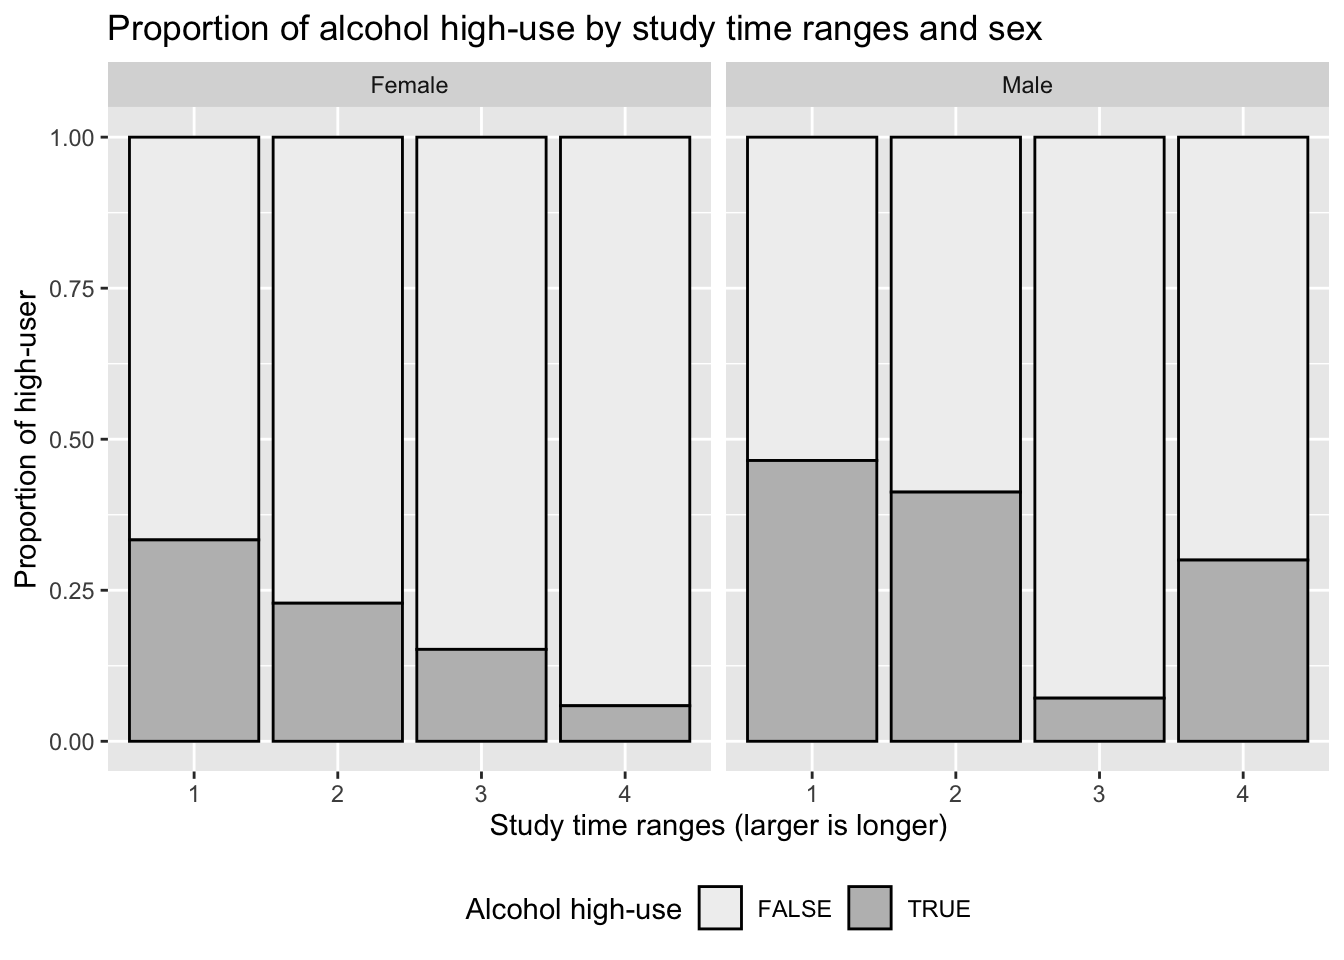
\includegraphics{chapter4_files/figure-latex/unnamed-chunk-29-1.pdf}
\caption{Fig. 8.3 Biplot of the LDA for separating clusters identified
by K means distance}
\end{figure}

\begin{verbatim}
## integer(0)
\end{verbatim}

\hypertarget{interpret-the-results-1}{%
\subsubsection{8.4 Interpret the
results}\label{interpret-the-results-1}}

Biplot based on LD1 and LD2 was generated, see fig 8.3. The three
clusters separated very clearly and some overlap observed between
cluster 1 and cluster 3, and between cluster 2 and cluster 3. Cluster 1
and cluster 2 are perfectly separated.

Based on arrows, variables rm, dis and crim explained more for cluster
1; variables indus, rad, tax and nox explained more for cluster 2; and
variables black, chas and ptratio explained more for clusters 3. Other
variables' role in clustering was much weaker.

\hypertarget{super-bonus-run-the-code-below-for-the-scaled-train-data-that-you-used-to-fit-the-lda.-the-code-creates-a-matrix-product-which-is-a-projection-of-the-data-points.-install-and-access-the-plotly-package.-create-a-3d-plot-of-the-columns-of-the-matrix-product-using-the-given-code.-adjust-the-code-add-argument-color-as-a-argument-in-the-plot_ly-function.-set-the-color-to-be-the-crime-classes-of-the-train-set.-draw-another-3d-plot-where-the-color-is-defined-by-the-clusters-of-the-k-means.-how-do-the-plots-differ-are-there-any-similarities-0-3-points-to-compensate-any-loss-of-points-from-the-above-exercises}{%
\subsection{9 Super-Bonus: Run the code below for the (scaled) train
data that you used to fit the LDA. The code creates a matrix product,
which is a projection of the data points. Install and access the plotly
package. Create a 3D plot of the columns of the matrix product using the
given code. Adjust the code: add argument color as a argument in the
plot\_ly() function. Set the color to be the crime classes of the train
set. Draw another 3D plot where the color is defined by the clusters of
the k-means. How do the plots differ? Are there any similarities? (0-3
points to compensate any loss of points from the above
exercises)}\label{super-bonus-run-the-code-below-for-the-scaled-train-data-that-you-used-to-fit-the-lda.-the-code-creates-a-matrix-product-which-is-a-projection-of-the-data-points.-install-and-access-the-plotly-package.-create-a-3d-plot-of-the-columns-of-the-matrix-product-using-the-given-code.-adjust-the-code-add-argument-color-as-a-argument-in-the-plot_ly-function.-set-the-color-to-be-the-crime-classes-of-the-train-set.-draw-another-3d-plot-where-the-color-is-defined-by-the-clusters-of-the-k-means.-how-do-the-plots-differ-are-there-any-similarities-0-3-points-to-compensate-any-loss-of-points-from-the-above-exercises}}

\hypertarget{run-the-code-below-for-the-scaled-train-data-that-you-used-to-fit-the-lda.-the-code-creates-a-matrix-product-which-is-a-projection-of-the-data-points.}{%
\subsubsection{9.1 Run the code below for the (scaled) train data that
you used to fit the LDA. The code creates a matrix product, which is a
projection of the data
points.}\label{run-the-code-below-for-the-scaled-train-data-that-you-used-to-fit-the-lda.-the-code-creates-a-matrix-product-which-is-a-projection-of-the-data-points.}}

\begin{Shaded}
\begin{Highlighting}[]
\CommentTok{\#reload the data}
\NormalTok{bos.s }\OtherTok{\textless{}{-}} \FunctionTok{as.data.frame}\NormalTok{(}\FunctionTok{scale}\NormalTok{(Boston))}
\CommentTok{\#generate cutoff according to quantile}
\NormalTok{bins }\OtherTok{\textless{}{-}} \FunctionTok{quantile}\NormalTok{(bos.s}\SpecialCharTok{$}\NormalTok{crim)}
\CommentTok{\#generate a categorical variable "crime" and re{-}code it}
\NormalTok{bos.s }\OtherTok{\textless{}{-}}\NormalTok{ bos.s }\SpecialCharTok{\%\textgreater{}\%} 
  \FunctionTok{mutate}\NormalTok{(}\AttributeTok{crime =}\NormalTok{ crim }\SpecialCharTok{\%\textgreater{}\%} 
           \FunctionTok{cut}\NormalTok{(}\AttributeTok{breaks =}\NormalTok{ bins, }\AttributeTok{include.lowest =} \ConstantTok{TRUE}\NormalTok{) }\SpecialCharTok{\%\textgreater{}\%} 
           \FunctionTok{fct\_recode}\NormalTok{(}\StringTok{"Low"} \OtherTok{=} \StringTok{"[{-}0.419,{-}0.411]"}\NormalTok{,}
                     \StringTok{"MediumLow"} \OtherTok{=} \StringTok{"({-}0.411,{-}0.39]"}\NormalTok{,}
                     \StringTok{"MediumHigh"} \OtherTok{=} \StringTok{"({-}0.39,0.00739]"}\NormalTok{,}
                     \StringTok{"High"} \OtherTok{=} \StringTok{"(0.00739,9.92]"}\NormalTok{))}
\CommentTok{\#remove crim}
\NormalTok{bos.s }\OtherTok{\textless{}{-}}\NormalTok{ bos.s }\SpecialCharTok{\%\textgreater{}\%} \FunctionTok{select}\NormalTok{(}\SpecialCharTok{{-}}\NormalTok{crim)}
\FunctionTok{set.seed}\NormalTok{(}\DecValTok{2022}\NormalTok{)}
\CommentTok{\#generate an object containing the number of observations}
\NormalTok{n }\OtherTok{\textless{}{-}}  \FunctionTok{nrow}\NormalTok{(bos.s)}
\CommentTok{\#generate a random set of indexing number with n = 80\% of the obs.}
\NormalTok{ind }\OtherTok{\textless{}{-}} \FunctionTok{sample}\NormalTok{(}\DecValTok{1}\SpecialCharTok{:}\NormalTok{n, }\AttributeTok{size =}\NormalTok{ n}\SpecialCharTok{*}\FloatTok{0.8}\NormalTok{)}
\CommentTok{\#generate the train set and test }
\NormalTok{train }\OtherTok{\textless{}{-}}\NormalTok{ bos.s[ind,]}
\NormalTok{test }\OtherTok{\textless{}{-}}\NormalTok{ bos.s[}\SpecialCharTok{{-}}\NormalTok{ind,]}
\end{Highlighting}
\end{Shaded}

\hypertarget{install-and-access-the-plotly-package.-create-a-3d-plot-of-the-columns-of-the-matrix-product-using-the-given-code.-adjust-the-code-add-argument-color-as-a-argument-in-the-plot_ly-function.-set-the-color-to-be-the-crime-classes-of-the-train-set.}{%
\subsubsection{9.2 Install and access the plotly package. Create a 3D
plot of the columns of the matrix product using the given code. Adjust
the code: add argument color as a argument in the plot\_ly() function.
Set the color to be the crime classes of the train
set.}\label{install-and-access-the-plotly-package.-create-a-3d-plot-of-the-columns-of-the-matrix-product-using-the-given-code.-adjust-the-code-add-argument-color-as-a-argument-in-the-plot_ly-function.-set-the-color-to-be-the-crime-classes-of-the-train-set.}}

\begin{Shaded}
\begin{Highlighting}[]
\CommentTok{\#select predictors for train set, with outcome variable removed}
\NormalTok{model\_predictors }\OtherTok{\textless{}{-}}\NormalTok{ dplyr}\SpecialCharTok{::}\FunctionTok{select}\NormalTok{(train, }\SpecialCharTok{{-}}\NormalTok{crime)}

\CommentTok{\# check the dimensions}
\FunctionTok{dim}\NormalTok{(model\_predictors)}
\end{Highlighting}
\end{Shaded}

\begin{verbatim}
## [1] 404  13
\end{verbatim}

\begin{Shaded}
\begin{Highlighting}[]
\FunctionTok{dim}\NormalTok{(lda.fit}\SpecialCharTok{$}\NormalTok{scaling)}
\end{Highlighting}
\end{Shaded}

\begin{verbatim}
## [1] 13  3
\end{verbatim}

\begin{Shaded}
\begin{Highlighting}[]
\CommentTok{\# matrix multiplication, saving the resulting matrix into matrix\_product}
\NormalTok{matrix\_product }\OtherTok{\textless{}{-}} \FunctionTok{as.matrix}\NormalTok{(model\_predictors) }\SpecialCharTok{\%*\%}\NormalTok{ lda.fit}\SpecialCharTok{$}\NormalTok{scaling}
\CommentTok{\#turn matrix into data frame}
\NormalTok{matrix\_product }\OtherTok{\textless{}{-}} \FunctionTok{as.data.frame}\NormalTok{(matrix\_product)}

\CommentTok{\#plot the 3D plot with LD1, LD2 and LD3}
\FunctionTok{library}\NormalTok{(plotly)}
\end{Highlighting}
\end{Shaded}

\begin{verbatim}
## 
## Attaching package: 'plotly'
\end{verbatim}

\begin{verbatim}
## The following object is masked from 'package:ggplot2':
## 
##     last_plot
\end{verbatim}

\begin{verbatim}
## The following object is masked from 'package:MASS':
## 
##     select
\end{verbatim}

\begin{verbatim}
## The following object is masked from 'package:stats':
## 
##     filter
\end{verbatim}

\begin{verbatim}
## The following object is masked from 'package:graphics':
## 
##     layout
\end{verbatim}

\begin{Shaded}
\begin{Highlighting}[]
\NormalTok{p1 }\OtherTok{\textless{}{-}} \FunctionTok{plot\_ly}\NormalTok{(}\AttributeTok{x =}\NormalTok{ matrix\_product}\SpecialCharTok{$}\NormalTok{LD1, }
        \AttributeTok{y =}\NormalTok{ matrix\_product}\SpecialCharTok{$}\NormalTok{LD2, }
        \AttributeTok{z =}\NormalTok{ matrix\_product}\SpecialCharTok{$}\NormalTok{LD3, }
        \AttributeTok{type=} \StringTok{\textquotesingle{}scatter3d\textquotesingle{}}\NormalTok{, }
        \AttributeTok{mode=}\StringTok{\textquotesingle{}markers\textquotesingle{}}\NormalTok{, }
        \AttributeTok{color =}\NormalTok{ train}\SpecialCharTok{$}\NormalTok{crime, }\CommentTok{\#Set the color to be the crime classes of the train set. }
        \AttributeTok{size =} \DecValTok{2}\NormalTok{)}
\NormalTok{p1}
\end{Highlighting}
\end{Shaded}

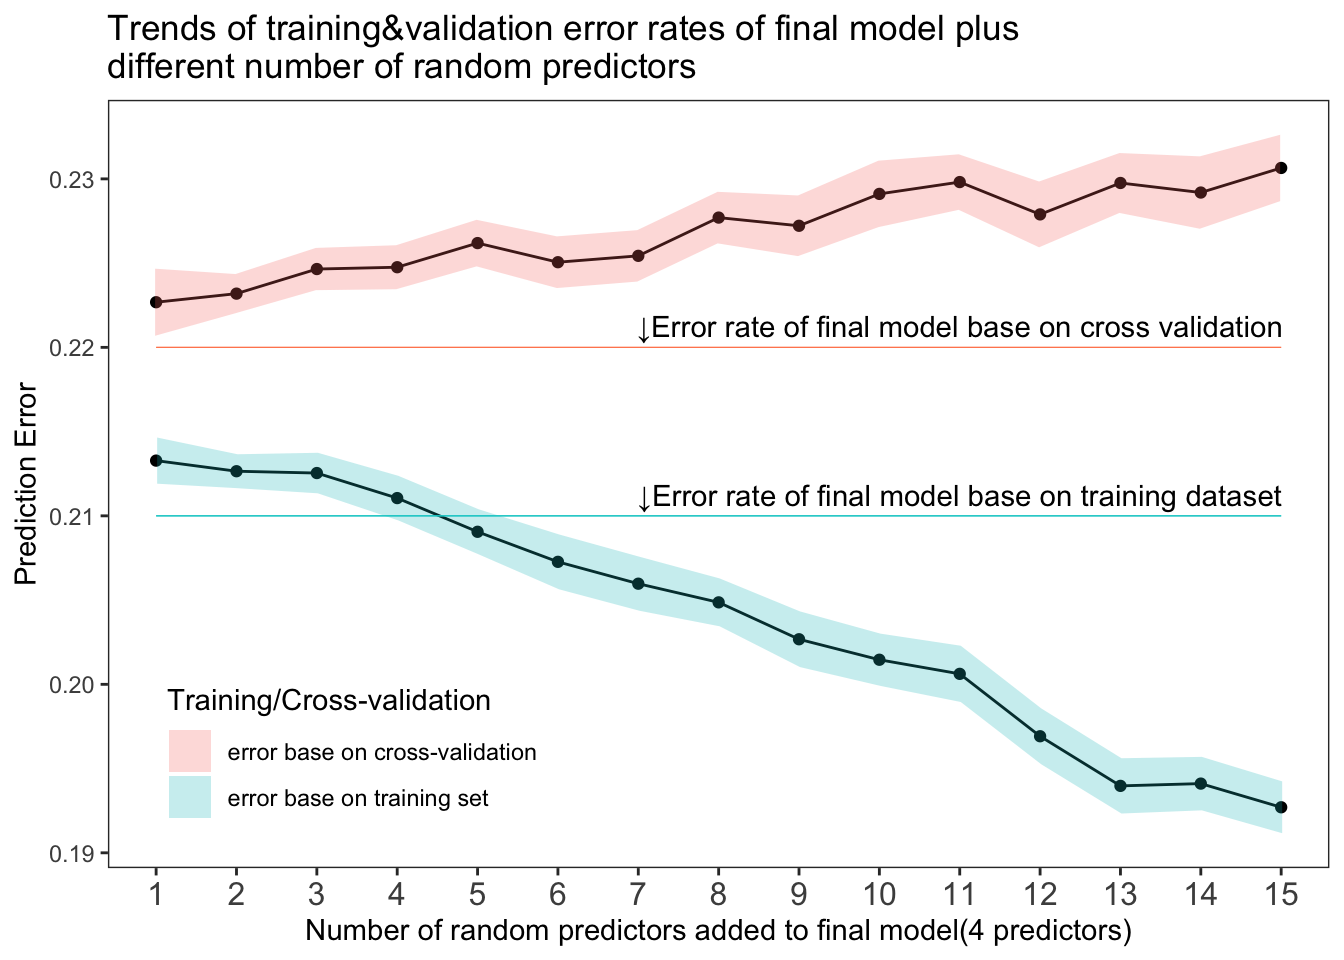
\includegraphics{chapter4_files/figure-latex/unnamed-chunk-31-1.pdf}

\hypertarget{draw-another-3d-plot-where-the-color-is-defined-by-the-clusters-of-the-k-means.}{%
\subsubsection{9.3 Draw another 3D plot where the color is defined by
the clusters of the
k-means.}\label{draw-another-3d-plot-where-the-color-is-defined-by-the-clusters-of-the-k-means.}}

\begin{Shaded}
\begin{Highlighting}[]
\CommentTok{\#select predictors for train set, with outcome variable removed}
\NormalTok{model\_predictors }\OtherTok{\textless{}{-}}\NormalTok{ dplyr}\SpecialCharTok{::}\FunctionTok{select}\NormalTok{(train, }\SpecialCharTok{{-}}\NormalTok{crime)}

\CommentTok{\#get the clusters of k{-}means for the train set}
\NormalTok{train.km }\OtherTok{\textless{}{-}} \FunctionTok{kmeans}\NormalTok{(model\_predictors, }\AttributeTok{centers =} \DecValTok{3}\NormalTok{) }


\NormalTok{p2 }\OtherTok{\textless{}{-}} \FunctionTok{plot\_ly}\NormalTok{(}\AttributeTok{x =}\NormalTok{ matrix\_product}\SpecialCharTok{$}\NormalTok{LD1, }
        \AttributeTok{y =}\NormalTok{ matrix\_product}\SpecialCharTok{$}\NormalTok{LD2, }
        \AttributeTok{z =}\NormalTok{ matrix\_product}\SpecialCharTok{$}\NormalTok{LD3, }
        \AttributeTok{type=} \StringTok{\textquotesingle{}scatter3d\textquotesingle{}}\NormalTok{, }
        \AttributeTok{mode=}\StringTok{\textquotesingle{}markers\textquotesingle{}}\NormalTok{, }
        \AttributeTok{color =} \FunctionTok{factor}\NormalTok{(train.km}\SpecialCharTok{$}\NormalTok{cluster), }\CommentTok{\#color defined by clusters of the k{-}means}
        \AttributeTok{size =} \FloatTok{1.5}\NormalTok{)}
\NormalTok{p2}
\end{Highlighting}
\end{Shaded}

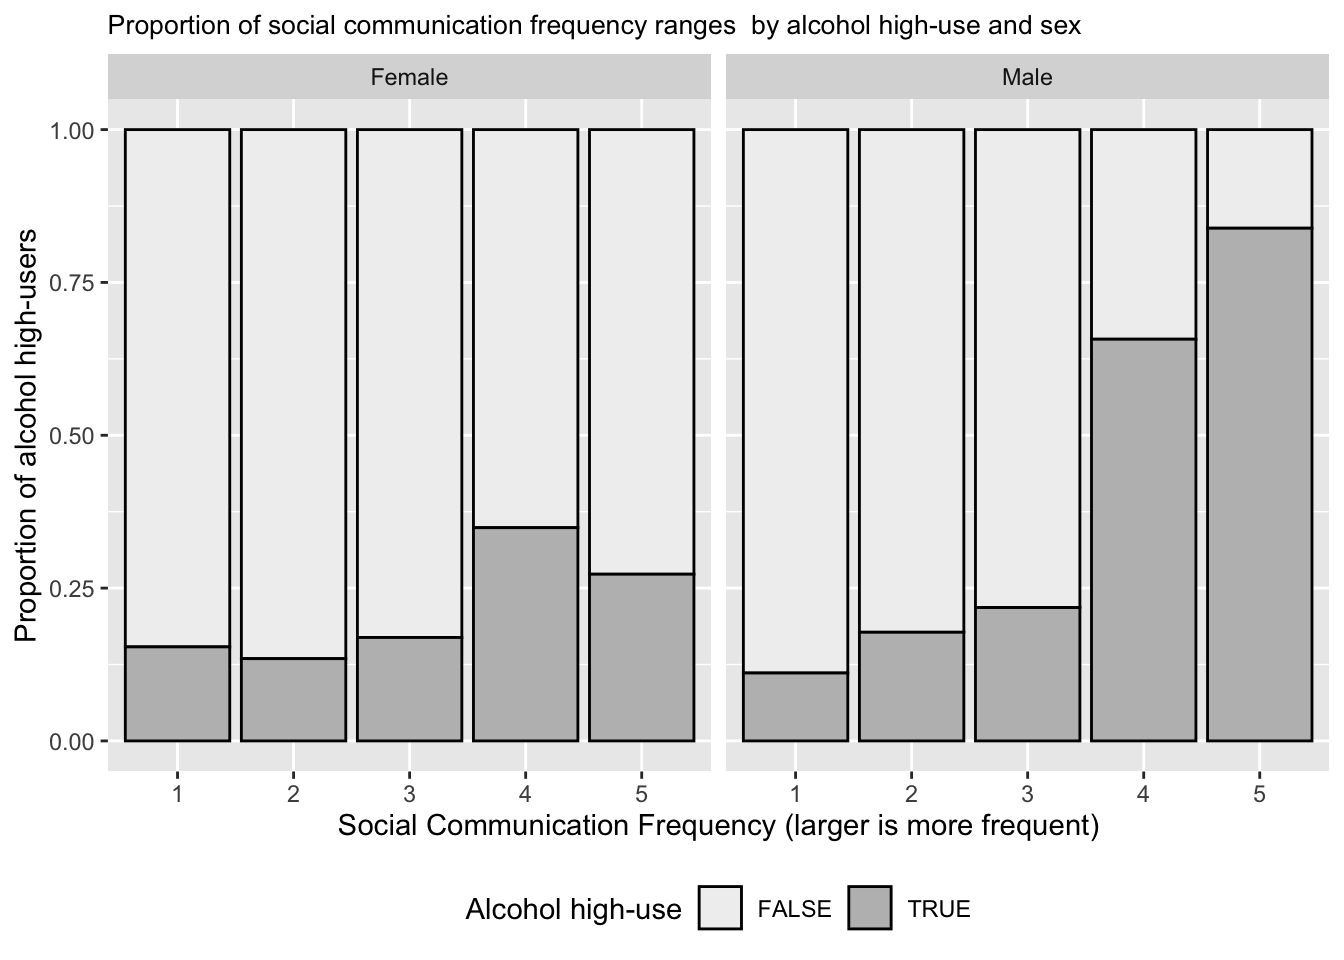
\includegraphics{chapter4_files/figure-latex/unnamed-chunk-32-1.pdf}

\hypertarget{how-do-the-plots-differ-are-there-any-similarities}{%
\subsubsection{9.4 How do the plots differ? Are there any
similarities?}\label{how-do-the-plots-differ-are-there-any-similarities}}

The LDA was trained according to a mathematical category of crime rates
(quantiles), which has 4 categories. While k = 3 was adopted for the
k-means clustering base on the size of within-cluster sum of square.
Since LDA is a supervised technique, we know what are each categories
represent, which are also labeled in the caption. K-means clustering is
a unsupervised method and thus I do not know anything about the
real-world representation of the 3 clusters identified before observing
closely.

However, by observing the pictures together, it is interesting to find
out that, cluster 3 from k-means nicely overlaps with High category from
LDA. Also, cluster 2 from k-means roughly overlaps with Low and Medium
low categories from LDA. As such, I will re-code categories from LDA
according to this finding and see closely on how well results from
k-means and LDA are consistent.

\hypertarget{recode-categories-from-lda-into-high-medium-and-low-old-low-medium-low}{%
\paragraph{9.4.1 Recode categories from LDA into High, Medium and Low
(old Low + Medium
Low)}\label{recode-categories-from-lda-into-high-medium-and-low-old-low-medium-low}}

\begin{Shaded}
\begin{Highlighting}[]
\NormalTok{train.crime3 }\OtherTok{\textless{}{-}}\NormalTok{ train }\SpecialCharTok{\%\textgreater{}\%} 
  \FunctionTok{mutate}\NormalTok{(}\AttributeTok{crime3 =}\NormalTok{ crime }\SpecialCharTok{\%\textgreater{}\%} 
           \FunctionTok{fct\_recode}\NormalTok{(}\StringTok{"Medium"} \OtherTok{=} \StringTok{"MediumHigh"}\NormalTok{ ,}
                      \StringTok{"Low"} \OtherTok{=} \StringTok{"MediumLow"}\NormalTok{,}
                      \StringTok{"High"} \OtherTok{=} \StringTok{"High"}\NormalTok{,}
                      \StringTok{"Low"} \OtherTok{=} \StringTok{"Low"}\NormalTok{))}

\NormalTok{km.cluster }\OtherTok{\textless{}{-}} \FunctionTok{factor}\NormalTok{(train.km}\SpecialCharTok{$}\NormalTok{cluster)}
\FunctionTok{levels}\NormalTok{(km.cluster) }\OtherTok{\textless{}{-}} \FunctionTok{c}\NormalTok{(}\StringTok{"Medium"}\NormalTok{,}\StringTok{"Low"}\NormalTok{,}\StringTok{"High"}\NormalTok{)}
\end{Highlighting}
\end{Shaded}

\hypertarget{check-the-accuracy-table}{%
\paragraph{9.4.2 Check the accuracy
table}\label{check-the-accuracy-table}}

\begin{Shaded}
\begin{Highlighting}[]
\NormalTok{accuracy.tab }\OtherTok{\textless{}{-}} \FunctionTok{table}\NormalTok{(}\AttributeTok{correct =}\NormalTok{ train.crime3}\SpecialCharTok{$}\NormalTok{crime3, }\AttributeTok{kmean.pred =}\NormalTok{ km.cluster)}
\NormalTok{accuracy.tab }
\end{Highlighting}
\end{Shaded}

\begin{verbatim}
##         kmean.pred
## correct  Medium Low High
##   Low         1  28  183
##   Medium      4  49   42
##   High       31  66    0
\end{verbatim}

\hypertarget{calculate-the-accuracy-rate}{%
\paragraph{9.4.3 Calculate the accuracy
rate}\label{calculate-the-accuracy-rate}}

\begin{Shaded}
\begin{Highlighting}[]
\CommentTok{\# looping through the 3X3 matrix to add up the columns and rows with same name}
\NormalTok{correct.n }\OtherTok{=} \DecValTok{0}
\ControlFlowTok{for}\NormalTok{ (i }\ControlFlowTok{in} \DecValTok{1}\SpecialCharTok{:}\DecValTok{3}\NormalTok{)\{}
\NormalTok{  correct.c }\OtherTok{\textless{}{-}}\NormalTok{ accuracy.tab[}\FunctionTok{which}\NormalTok{(}\FunctionTok{rownames}\NormalTok{(accuracy.tab) }\SpecialCharTok{==} \FunctionTok{colnames}\NormalTok{(accuracy.tab)[i]), i]}
\NormalTok{  correct.n }\OtherTok{=}\NormalTok{ correct.c}\SpecialCharTok{+}\NormalTok{ correct.n}
\NormalTok{\} }
\CommentTok{\# calculate the accuracy rate}
\NormalTok{correct.n}\SpecialCharTok{/}\NormalTok{(}\FunctionTok{nrow}\NormalTok{(bos.s)}\SpecialCharTok{*}\FloatTok{0.8}\NormalTok{)}
\end{Highlighting}
\end{Shaded}

\begin{verbatim}
## [1] 0.07905138
\end{verbatim}

It gets an accuracy rate of 71.3\%, greatly outperforming the original
LDA model, indicating k-mean cluster could be used as a cue for
categorizing continuous variables.

\end{document}
